\setchapterimage[8cm]{Paul Pastourmatzis Unsplash}
\setchapterpreamble[u]{\margintoc}
\chapter{数学分析III}
\labch{mathematical_analysis_3}

\section{多元微分学}

在\cite{邓东皋} 中,$f_{xy}$表示$\frac{\partial}{\partial y}\frac{\partial f}{\partial x}$. 即先对$x$求偏导,再对$y$求偏导.这一点与\cite{崔尚斌}不同,也和主流教材不同.

\subsection{多元函数的极值}

\begin{theorem}[Hessian判别法]\label{thm:hessian-discrimination}
    如果Hessian矩阵在$x$处是正定的,那么$f$在$x$处取得孤立的局部极小值。如果Hessian矩阵在$x$处是负定的,那么$f$在$x$处取得孤立的局部极大值。如果Hessian矩阵有正有负的特征值,那么$x$是$f$的鞍点。否则,该测试是不确定的。这意味着在局部极小值处,Hessian矩阵是正半定的,而在局部极大值处,Hessian矩阵是负半定的。

    对于正半定和负半定的Hessian矩阵,该测试是不确定的(在Hessian矩阵是半定但不是定的临界点可能是局部极值或鞍点)。然而,从Morse理论的角度可以得出更多结论。
\end{theorem}

\subsection{偏导数}
\begin{theorem}[杨定理]
    设函数 $f(x, y)$ 在点 $\left(x_0, y_0\right)$ 的某个邻域上有定义,且在此邻域上存在偏导数。假设两个偏导数 $f_x$ 和 $f_y$ 都在点 $\left(x_0, y_0\right)$ 可微,则
$$
\frac{\partial^2 f}{\partial x \partial y}\left(x_0, y_0\right)=\frac{\partial^2 f}{\partial y \partial x}\left(x_0, y_0\right) .
$$
\end{theorem}

\begin{proof}
    证明 考虑一元函数
$$
g(h)=f\left(x_0+h, y_0+h\right)-f\left(x_0+h, y_0\right)-f\left(x_0, y_0+h\right)+f\left(x_0, y_0\right) .
$$
我们来证明
\begin{align}
g(h)=f_{y x}\left(x, y_0\right) h^2+o\left(h^2\right), & \text { 当 } h \rightarrow 0,\label{eq:g-h-1} \\
g(h)=f_{x y}\left(x, y_0\right) h^2+o\left(h^2\right), & \text { 当 } h \rightarrow 0.\label{eq:g-h-2}
\end{align}
显然,所要证明的结论是式(\ref{eq:g-h-1})和式(\ref{eq:g-h-2})的直接推论。
对每个固定的充分小的 $h \neq 0$ ,考虑一元函数
$$
\varphi(x)=f\left(x, y_0+h\right)-f\left(x, y_0\right)
$$
显然有
$$
g(h)=\varphi\left(x_0+h\right)-\varphi\left(x_0\right) .
$$
对这个表达式应用拉格朗日中值定理可知存在 $0<\theta_1<1$ 使
\begin{equation}\label{eq:g-h-3}
    g(h)=\varphi^{\prime}\left(x_0+\theta_1 h\right) h=\left[f_x\left(x_0+\theta_1 h, y_0+h\right)-f_x\left(x_0+\theta_1 h, y_0\right)\right] h .
\end{equation}
由于 $f_x$ 在点 $\left(x_0, y_0\right)$ 可微,所以
$$
\begin{aligned}
f_x\left(x_0+\theta_1 h, y_0+h\right) & =f_x\left(x_0, y_0\right)+f_{x x}\left(x_0, y_0\right) \theta_1 h+f_{y x}\left(x_0, y_0\right) h+o(h), \quad \text { 当 } h \rightarrow 0, \\
f_x\left(x_0+\theta_1 h, y_0\right) & =f_x\left(x_0, y_0\right)+f_{x x}\left(x_0, y_0\right) \theta_1 h+o(h), \quad \text { 当 } h \rightarrow 0 .
\end{aligned}
$$
把这两个等式代入式(\ref{eq:g-h-3}),就得到了式(\ref{eq:g-h-1}).同理,通过考虑一元函数
$$
\psi(y)=f\left(x_0+h, y\right)-f\left(x_0, y\right)
$$
便可证明式(\ref{eq:g-h-2}).证毕.
\end{proof}



\subsection{泰勒公式}
\begin{theorem}[泰勒公式]
    设 $D$ 是 $\mathbf{R}^m$ 中的凸区域,$x_0$ 是 $D$ 中一点.又设 $f$ 是在 $D$ 上 $n+1$ 阶可微的函数.则对任意 $x \in D$ ,存在位于 $x_0$ 和 $x$ 的连线上的点 $\xi$ 使
$$
f(x)=\sum_{|\alpha| \leqslant n} \frac{1}{\alpha!} \partial^\alpha f\left(x_0\right)\left(x-x_0\right)^\alpha+\sum_{|\alpha|=n+1} \frac{1}{\alpha!} \partial^\alpha f(\xi)\left(x-x_0\right)^\alpha .
$$
等式右端的第一个和号 $\sum_{|\alpha| \leqslant n}$ 表示关于所有满足条件 $|\alpha| \leqslant n$ 的 $m$ 重指标 $\alpha \in \mathbf{Z}_{+}^m$ 求
和,第二个和号 $\sum_{|\alpha|=n+1}$ 则表示关于所有满足条件 $|\alpha|=n+1$ 的 $m$ 重指标 $\alpha \in \mathbf{Z}_{+}^m$ 求和.
\end{theorem}


\section{积分的交换次序问题}

设$I$是一个任意类型的区间(闭区间、开区间、半开半闭区间、无穷区间).

\begin{theorem}[极限与积分交换次序]\label{thm:limit-and-integral-exchange}
    设函数$f(x,y)$在$I\times [c,d]$上连续,则对于任意$x_0\in I$,有
    \[
        \lim_{\substack{x\to x_0\\x\in I}}\int_c^d f(x,y)\mathrm{d} y = \int_c^d \lim_{\substack{x\to x_0\\x\in I}}f(x,y)\mathrm{d} y
    \]
    即函数$g(x)=\int_c^d f(x,y)\mathrm{d} y$在$I$上连续.
\end{theorem}

\begin{proof}
    用$\varepsilon$-$\delta$语言\sidenote[][*2]{借助$f$自身的连续性,连续是一个局部的性质,所以不管$I$是什么类型的区间都行.},照章办事.
\end{proof}

\begin{theorem}[导数与积分交换次序]\label{thm:derivative-and-integral-exchange}
    $f(x,y)$是定义在$I\times [c,d]$上的函数,且满足以下两个条件:
    \begin{enumerate}
        \item 对每个$x\in I$,$f(x,y)$作为$y$的函数在$[c,d]$上可积;
        \item $f(x,y)$关于$x$有偏导数,且偏导数$f_x(x,y)$在$I\times [c,d]$上连续.
    \end{enumerate}
    则$F(x)=\int_c^d f(x,y)\mathrm{d} y$在$x\in I$上可导,且
    \[
        F'(x)=\int_c^d \frac{\partial f(x,y)}{\partial x}\mathrm{d} y
    \]
\end{theorem}

\begin{proof}
    \begin{align*}
        \left|\frac{g(x)-g\left(x_0\right)}{x-x_0}-\int_c^d f_x\left(x_0, y\right) \mathrm{d} y\right| &\leqslant \int_c^d\left|\frac{f(x, y)-f\left(x_0, y\right)}{x-x_0}-f_x\left(x_0, y\right)\right| \mathrm{d} y \\
        &=O(|x-x_0|)
    \end{align*}
\end{proof}

\begin{theorem}[积分交换次序]\label{thm:integral-exchange}
    设$f(x,y)$在$[a,b]\times [c,d]$上连续,则
    \[
        \int_a^b\left(\int_c^d f(x,y)\mathrm{d} y\right)\mathrm{d} x = \int_c^d\left(\int_a^b f(x,y)\mathrm{d} x\right)\mathrm{d} y
    \]
\end{theorem}

\begin{proof}
    考虑函数
    \[
    g(x,t)=\int_c^t f(x,y)\mathrm{d} y,\quad x\in[a,b],\quad t\in[c,d]
    \]
    由$f$连续性可知,$g(x,t)$关于$t$有偏导数,且
    \[
        g_t(x,t)=f(x,t),\quad x\in[a,b],\quad t\in[c,d]
    \]
    由定理\ref{thm:derivative-and-integral-exchange}可知
    \[
    \frac{\mathrm{d}}{\mathrm{d}t}\int_a^b g(x,t) \mathrm{d}x=\int_a^b g_t(x,t) \mathrm{d}x=\int_a^b f(x,t) \mathrm{d}x,\quad \forall t\in[c,d]
    \]
    这说明,函数$t\mapsto \int_a^b g(x,t)\mathrm{d}x$是函数$x\mapsto \int_a^b f(x,t)\mathrm{d}x$的原函数,因此根据牛顿-莱布尼茨公式,有
    \[
        \int_c^d \left(\int_a^b f(x,y)\mathrm{d} x\right)\mathrm{d} y = \int_a^b \left(\int_c^d f(x,y)\mathrm{d} y\right)\mathrm{d} x
    \]
\end{proof}

\begin{theorem}[含参积分求导公式]\label{thm:derivative-of-integral-with-parameter}
    设$f$与$D_2f$在矩形$[a,b]\times [c,d]$上连续,设$p,q$在$[c,d]$上可微,且$p,q\in[a,b]$,则
    \[
        D_2\int_{p(y)}^{q(y)} f(x,y)\mathrm{d} x = \int_{p(y)}^{q(y)} D_2f(x,y)\mathrm{d} x +f(q(y),y)q'(y)-f(p(y),y)p'(y)
    \]
\end{theorem}

\begin{proof}
    设$G(x_1,x_2,x_3)=\int_{x_1}^{x_2}f(t,x_3)\mathrm{d} t$,再利用求导的链式法则即可.
\end{proof}

\section{含参变量广义积分}

\subsection{含参变量广义积分的一致收敛}

见\cite{崔尚斌} p.151.
\begin{theorem}[一致收敛的柯西准则]
    无穷积分 $\int_c^{+\infty} f(x, y) \mathrm{d} y$ 关于 $x \in I$ 一致收玫的充要条件是,对任意给定的 $\varepsilon>0$ ,存在相应的 $A>c$ ,使当 $d_1, d_2>A$ 时,对所有 $x \in[a, b]$ 都成立
$$
\left|\int_{d_1}^{d_2} f(x, y) \mathrm{d} y\right|<\varepsilon
$$
\end{theorem}
\begin{theorem}[魏尔斯特拉斯 $M$ 判别法]
    设存在定义在 $[c,+\infty)$ 上的非负连续函数 $M(y)$ 使成立
$$
|f(x, y)| \leqslant M(y), \quad \forall x \in I, \quad \forall y \geqslant c
$$
并且广义积分 $\int_c^{+\infty} M(y) \mathrm{d} y$ 收敛,则广义积分 $\int_c^{+\infty} f(x, y) \mathrm{d} y$ 关于 $x \in I$ 一致收敛.
\end{theorem}
\begin{theorem}[狄利克雷判别法]
    设
    \begin{enumerate}
        \item 函数 $d \mapsto \int_c^d f(x, y) \mathrm{d} y$ 关于 $x \in I$ 一致有界,即存在常数 $M>0$ 使成立
$$
\left|\int_c^d f(x, y) \mathrm{d} y\right| \leqslant M, \quad \forall x \in I, \quad \forall d \geqslant c
$$
        \item 对每个固定的 $x \in I$ ,函数 $g(x, y)$ 关于 $y$ 是单调的,并且当 $y \rightarrow+\infty$ 时, $g(x, y)$ 关于 $x \in I$ 一致地收玫于零,即对任意给定的 $\varepsilon>0$ ,存在相应的 $d>c$ ,使得
$$
|f(x, y)|<\varepsilon, \quad \forall x \in I, \quad \forall y>d
$$
    \end{enumerate}
则广义积分 $\int_c^{+\infty} f(x, y) g(x, y) \mathrm{d} y$ 关于 $x \in I$ 一致收敛.
\end{theorem}
\begin{theorem}[阿贝尔判别法]
    设
    \begin{enumerate}
        \item 广义积分 $\int_c^{+\infty} f(x, y) \mathrm{d} y$ 关于 $x \in I$ 一致收敛.
        \item 对每个固定的 $x \in I$ ,函数 $g(x, y)$ 关于 $y$ 是单调的,并且作为 $y$ 的函数,$g(x, y)$关于 $x \in I$ 一致有界,即存在常数 $M>0$ 使成立
$$
|g(x, y)| \leqslant M, \quad \forall x \in I, \quad \forall y \geqslant c .
$$
    \end{enumerate}
则广义积分 $\int_c^{+\infty} f(x, y) g(x, y) \mathrm{d} y$ 关于 $x \in I$ 一致收敛.
\end{theorem}

\begin{exercise}
    证明无穷积分 $\int_0^{+\infty} \frac{\sin x}{x} \mathrm{e}^{-t x} \mathrm{~d} x$ 关于 $t \geqslant 0$ 一致收敛.
\end{exercise}

\begin{proof}
    无穷积分 $\int_0^{+\infty} \frac{\sin x}{x} \mathrm{~d} x$ 是收敛的 (见 9.1 节例 11). 又对每个固定的 $t \geqslant 0$,函数 $\mathrm{e}^{-t x}$ 关于 $x$ 是单调的, 并且
    \[
    \left|\mathrm{e}^{-t x}\right| \leqslant 1, \quad \forall t \geqslant 0, \quad \forall x \geqslant 0 .
    \]
    所以由阿贝尔判别法知,无穷积分 $\int_0^{+\infty} \frac{\sin x}{x} \mathrm{e}^{-t x} \mathrm{~d} x$ 关于 $t \geqslant 0$ 一致收敛.
\end{proof}

接下来是一个证明不一致收敛\sidenote{所谓的不一致收敛,是一个与“一致收敛”相反的概念,这是一个逻辑学上的问题.}的例子:
\begin{example}
    对无穷积分 $I(\alpha)=\int_1^{+\infty} x^\alpha \mathrm{e}^{-x} \mathrm{~d} x$, 证明:
\begin{enumerate}
    \item 对任意 $a>0, I(\alpha)$ 关于 $0 \leqslant \alpha \leqslant a$ 一致收敛.
    \item $I(\alpha)$ 关于 $\alpha \geqslant 0$ 不一致收敛.
\end{enumerate}
\end{example}
\begin{proof}
    \begin{enumerate}
        \item 由于
        \[
        0 \leqslant x^\alpha \mathrm{e}^{-x} \leqslant x^a \mathrm{e}^{-x}, \quad \forall x \geqslant 1, \quad \forall \alpha \in[0, a],
        \]
        而无穷积分 $I(\alpha)=\int_1^{+\infty} x^a \mathrm{e}^{-x} \mathrm{~d} x$ 收敛, 所以由 $M$ 判别法知, $I(\alpha)$ 关于 $0 \leqslant \alpha \leqslant a$ 一致收敛.
        \item 由于
        \[
        \int_n^{+\infty} x^n \mathrm{e}^{-x} \mathrm{~d} x=-\left.x^n \mathrm{e}^{-x}\right|_n ^{+\infty}+n \int_n^{+\infty} x^{n-1} \mathrm{e}^{-x} \mathrm{~d} x \geqslant n^n \mathrm{e}^{-n} \geqslant \mathrm{e}^{-1}, \quad n=1,2, \cdots,
        \]
        所以 $I(\alpha)$ 关于 $\alpha \geqslant 0$ 不一致收敛.
\end{enumerate}
\end{proof}
\subsection{含参变量广义积分换序}
很多教材都没有说清楚这一点,但是\cite{崔尚斌} p.153. 有很好的说明. 他引入了“局部一致收敛”的概念,这是必要的.
\begin{definition}[局部一致收敛]
    设对每个给定的 $x \in I$, 无穷积分 $\int_c^{+\infty} f(x, y) \mathrm{d} y$ 收敛. 如果对任意 $x_0 \in I$, 都存在相应的 $\delta>0$, 使得该无穷积分关于 $x \in I \bigcap\left[x_0-\delta, x_0+\delta\right]$ 一致收敛, 则称这个无穷积分关于 $x \in I$ \textcolor{red}{局部地一致收敛}.
\end{definition}
\begin{theorem}[极限和积分交换次序]\label{thm:limit-and-integral-exchange}
    设 $f(x, y)$ 在 $I \times[c,+\infty)$ 上连续, 且广义积分 $g(x)=\int_c^{+\infty} f(x, y) \mathrm{d} y$ 关于 $x \in I$ \textcolor{red}{局部地一致收敛}. 则对任意 $x_0 \in I$ 都成立
    \[
    \lim _{\substack{x \rightarrow x_0 \\ x \in I}} \int_c^{+\infty} f(x, y) \mathrm{d} y=\int_c^{+\infty} f\left(x_0, y\right) \mathrm{d} y=\int_c^{+\infty} \lim _{\substack{x \rightarrow x_0 \\ x \in I}} f(x, y) \mathrm{d} y,
    \]
    即函数 $g(x)=\int_c^{+\infty} f(x, y) \mathrm{d} y$ 在 $I$ 上连续.
\end{theorem}
\begin{proof}
    证明考虑三分法. 还要注意区分$x_0$是否是区间$I$的端点\sidenote{这是证明严谨性上的考量.}. 不过是否是端点的讨论是类似的.
\end{proof}
\begin{theorem}[积分交换次序]\label{thm:integral-exchange}
    设 $f(x, y)$ 在 $[a, b] \times[c,+\infty)$ 上连续, 且广义积分 $g(x)=\int_c^{+\infty} f(x, y) \mathrm{d} y$ 关于 $x \in[a, b]$ \textcolor{red}{一致收敛}\sidenote{注意这里积分是一个整体的概念,而求导是一个局部的概念,所以前者是一致收敛,后者是局部一致收敛.}. 则成立
    \[
    \int_a^b\left(\int_c^{+\infty} f(x, y) \mathrm{d} y\right) \mathrm{d} x=\int_c^{+\infty}\left(\int_a^b f(x, y) \mathrm{d} x\right) \mathrm{d} y .
    \]
\end{theorem}
\begin{proof}
    证明只需照章办事.
\end{proof}
接下来我们给出这一节最重要的定理.
\begin{theorem}[导数和积分交换次序]\label{thm:derivative-and-integral-exchange}
    对任意区间 $I$ 和定义在 $I \times[c,+\infty)$ 上的函数 $f(x, y)$, 设以下三个条件满足:
    \begin{enumerate}
        \item 对每个 $x \in I$, 广义积分 $g(x)=\int_c^{+\infty} f(x, y) \mathrm{d} y$ 收敛;
        \item $f(x, y)$ 关于变元 $x$ 有偏导数, 且偏导函数 $f_x(x, y)$ 在 $I \times[c,+\infty)$ 上连续;
        \item 广义积分 $\int_c^{+\infty} f_x(x, y) \mathrm{d} y$ 关于 $x \in I$ 局部地一致收敛。\sidenote{这个局部一致收敛不用考虑对$I$的端点!换言之,只用考虑开区间.}
    \end{enumerate}
    则函数 $g(x)=\int_c^{+\infty} f(x, y) \mathrm{d} y$ 在 $I$ 上可导, 且 $g^{\prime}(x)=\int_c^{+\infty} f_x(x, y) \mathrm{d} y$, 即导数和积分可以交换次序:
    \[
    \frac{\mathrm{d}}{\mathrm{~d} x} \int_c^{+\infty} f(x, y) \mathrm{d} y=\int_c^{+\infty} f_x(x, y) \mathrm{d} y=\int_c^{+\infty} \frac{\partial}{\partial x} f(x, y) \mathrm{d} y, \quad \forall x \in I .
    \]
    这里当 $x$ 是区间 $I$ 的端点时, 导数指的是单侧导数.
\end{theorem}
\begin{note}
    每当使用到积分和导数交换的时候,都要提一下这个定理,说明是可以交换的. 这个定理的证明也是比较很显然的,只需要在局部上使用定理\ref{thm:limit-and-integral-exchange}即可.
\end{note}
\begin{proof}
    令
    \[
    h(x)=\int_c^{+\infty} f_x(x, y) \mathrm{d} y, \quad \forall x \in I .
    \]
    根据定理 18.2.5, 从条件 (2) 和条件 (3) 推知 $h(x)$ 是 $I$ 上的连续函数. 进一步, 根据定理 18.2.6, 从条件 (2) 和条件 (3) 可知对任意 $s, t \in I(s<t)$ 成立
    \begin{align*}
        \int_s^t h(x) \mathrm{d} x & =\int_s^t\left(\int_c^{+\infty} f_x(x, y) \mathrm{d} y\right) \mathrm{d} x=\int_c^{+\infty}\left(\int_s^t f_x(x, y) \mathrm{d} x\right) \mathrm{d} y \\
    & =\int_c^{+\infty}[f(t, y)-f(s, y)] \mathrm{d} y=g(t)-g(s) .
    \end{align*}
    由上式和变限积分的导数定理(定理 7.3.4)知, $g(x)$ 在 $I$ 上可导,且 $g^{\prime}(x)=h(x)$ , $\forall x \in I$. 证毕.
\end{proof}
接下来给出一个应用的例子.
\begin{example}
    求狄利克雷积分 $\int_0^{+\infty} \frac{\sin x}{x} \mathrm{~d} x$.
\end{example}
\begin{note}
    利用积分与极限交换顺序\ref{thm:limit-and-integral-exchange}
\end{note}
\begin{solution}
    考虑含参量的广义积分
    \[
    g(t)=\int_0^{+\infty} \frac{\sin x}{x} \mathrm{e}^{-t x} \mathrm{~d} x, \quad t \geqslant 0 .
    \]
    由例 2 知这个广义积分关于 $t \in[0,+\infty)$ 一致收敛, 因而 $g(t)$ 是区间 $[0,+\infty)$ 上的连续函数. 易见
    \[
    g(0)=\int_0^{+\infty} \frac{\sin x}{x} \mathrm{~d} x,
    \]
    且
    \[
    |g(t)|=\left|\int_0^{+\infty} \frac{\sin x}{x} \mathrm{e}^{-t x} \mathrm{~d} x\right| \leqslant \int_0^{+\infty} \mathrm{e}^{-t x} \mathrm{~d} x=\frac{1}{t}, \quad \forall t>0,
    \]
    从而
    \[
    \lim _{t \rightarrow+\infty} g(t)=0 .
    \]
    如果关于 $t>0$ 的求导运算 (\textcolor{red}{注意不需要在 $t=0$ 处求导}) 能够与关于 $x$ 的无穷积分交换次序,那么有
    \[
    g^{\prime}(t)=\int_0^{+\infty}(\sin x) \mathrm{e}^{-t x} \mathrm{~d} x=\left.\frac{\mathrm{e}^{-t x}(t \sin x+\cos x)}{1+t^2}\right|_{x=0} ^{+\infty}=-\frac{1}{1+t^2}, \quad \forall t>0,
    \]
    进而对任意 $t>0$, 有
    \[
    g(t)-g(0)=-\int_0^t \frac{\mathrm{~d} \eta}{1+\eta^2}=-\left.\arctan \eta\right|_0 ^t=-\arctan t .
    \]
    令 $t \rightarrow+\infty$, 得
    \[
    g(0)=\lim _{t \rightarrow+\infty} \arctan t=\frac{\pi}{2} .
    \]
    因此,剩下的问题只是验证求导运算与无穷积分交换次序的条件是满足的. 而这只需证明, 积分号下求导所得到的广义积分 $h(t)=\int_0^{+\infty}(\sin x) \mathrm{e}^{-t x} \mathrm{~d} x$ 关于 $t \in(0,+\infty)$ 局部地一致收敛. 这个条件的确是满足的. 这是因为, 显然对任意 $a>0$, 有
    \[
    \left|(\sin x) \mathrm{e}^{-t x}\right| \leqslant \mathrm{e}^{-a x}, \quad \forall t \geqslant a, \quad \forall x \geqslant 0,
    \]
    所以运用 $M$ 判别法知, $h(t)$ 关于 $t \geqslant a$ 一致收敛. 由于对任意 $t_0>0$, 只要取 $\delta=\frac{t_0}{2}$ 和 $a=\frac{t_0}{2}$, 就有 $\left[t_0-\delta, t_0+\delta\right] \subseteq [\frac{t_0}{2},+\infty)$, 进而应用前述结论知 $h(t)$ 关于 $t \in\left[t_0-\delta, t_0+\delta\right]$一致收敛, 所以就证明了广义积分 $h(t)=\int_0^{+\infty}(\sin x) \mathrm{e}^{-t x} \mathrm{~d} x$ 关于 $t \in(0,+\infty)$ 局部地一致收敛.
\end{solution}
之前讨论的广义积分交换问题\ref{thm:integral-exchange},其中一个是定积分,接下来讨论两个积分都是广义积分的情况.
\begin{theorem}[定理 18.2.8]
    设 $f(x, y)$ 是 $[a,+\infty) \times[c,+\infty)$ 上的连续函数, 满足以下三个条件:
    \begin{enumerate}
        \item 对任意 $b>a$, 广义积分 $\int_c^{+\infty}|f(x, y)| \mathrm{d} y$ 关于 $x \in[a, b]$ 一致收敛;
        \item 对任意 $d>c$, 广义积分 $\int_a^{+\infty}|f(x, y)| \mathrm{d} x$ 关于 $y \in[c, d]$ 一致收敛;
        \item 两个广义积分
        \[
        \int_a^{+\infty}\left(\int_c^{+\infty}|f(x, y)| \mathrm{d} y\right) \mathrm{d} x \quad \text { 和 } \quad \int_c^{+\infty}\left(\int_a^{+\infty}|f(x, y)| \mathrm{d} x\right) \mathrm{d} y
        \]
    \end{enumerate}
    至少有一个收敛。则另一个广义积分也必收敛,而且成立以下等式:
    \[
    \begin{aligned}
    \int_a^{+\infty}\left(\int_c^{+\infty}|f(x, y)| \mathrm{d} y\right) \mathrm{d} x & =\int_c^{+\infty}\left(\int_a^{+\infty}|f(x, y)| \mathrm{d} x\right) \mathrm{d} y \\
    \int_a^{+\infty}\left(\int_c^{+\infty} f(x, y) \mathrm{d} y\right) \mathrm{d} x & =\int_c^{+\infty}\left(\int_a^{+\infty} f(x, y) \mathrm{d} x\right) \mathrm{d} y
    \end{aligned}
    \]
\end{theorem}
\begin{proof}
    证明只需照章办事. 首先由一致收敛性可知函数$\displaystyle x\mapsto\int_c^{+\infty}f(x,y)\mathrm{d}y$是$[a,+\infty)$上连续函数,因此可积,类似地,函数$\displaystyle y\mapsto\int_a^{+\infty}f(x,y)\mathrm{d}x$也是$[c,+\infty)$上连续函数,因此可积. 于是不妨设$\int_c^{+\infty}\left(\int_a^{+\infty} f(x, y) \mathrm{d} x\right) \mathrm{d} y$ 收敛. 故只需证
    \begin{equation}
        \lim _{b \rightarrow+\infty} \int_a^b\left(\int_c^{+\infty} f(x, y) \mathrm{d} y\right) \mathrm{d} x=\int_c^{+\infty}\left(\int_a^{+\infty} f(x, y) \mathrm{d} x\right) \mathrm{d} y.
    \end{equation}
    由于对每个 $b>a$, 广义积分 $\int_c^{+\infty} f(x, y) \mathrm{d} y$ 关于 $x \in[a, b]$ 一致收敛, 所以由定理 \ref{thm:limit-and-integral-exchange} 知
$$
\int_a^b\left(\int_c^{+\infty} f(x, y) \mathrm{d} y\right) \mathrm{d} x=\int_c^{+\infty}\left(\int_a^b f(x, y) \mathrm{d} x\right) \mathrm{d} y,
$$
    因此
    $$
\begin{aligned}
& \left|\int_a^b\left(\int_c^{+\infty} f(x, y) \mathrm{d} y\right) \mathrm{d} x-\int_c^{+\infty}\left(\int_a^{+\infty} f(x, y) \mathrm{d} x\right) \mathrm{d} y\right| \\
= & \left|\int_c^{+\infty}\left(\int_a^b f(x, y) \mathrm{d} x\right) \mathrm{d} y-\int_c^{+\infty}\left(\int_a^{+\infty} f(x, y) \mathrm{d} x\right) \mathrm{d} y\right|\\
& \leqslant \int_c^{+\infty}\left(\int_b^{+\infty}|f(x, y)| \mathrm{d} x\right) \mathrm{d} y \\
& =\int_c^d\left(\int_b^{+\infty}|f(x, y)| \mathrm{d} x\right) \mathrm{d} y+\int_d^{+\infty}\left(\int_b^{+\infty}|f(x, y)| \mathrm{d} x\right) \mathrm{d} y \\
& \leqslant \int_c^d\left(\int_b^{+\infty}|f(x, y)| \mathrm{d} x\right) \mathrm{d} y+\int_d^{+\infty}\left(\int_a^{+\infty}|f(x, y)| \mathrm{d} x\right) \mathrm{d} y \\
& \equiv A+B
\end{aligned}
$$
\begin{note}
    接下来照章办事,注意放缩的先后关系即可.
\end{note}
由于 $\int_c^{+\infty}\left(\int_a^{+\infty}|f(x, y)| \mathrm{d} x\right) \mathrm{d} y<\infty$, 所以对任意给定的 $\varepsilon>0$, 存在相应的 $N>c$,使对任意 $d>N$ 都有
$$
B=\int_d^{+\infty}\left(\int_a^{+\infty}|f(x, y)| \mathrm{d} x\right) \mathrm{d} y<\frac{\varepsilon}{2} .
$$
取定一个这样的 $d$. 因为广义积分 $\int_a^{+\infty}|f(x, y)| \mathrm{d} x$ 关于 $y \in[c, d]$ 一致收敛, 所以对给定的 $\varepsilon>0$, 存在相应的 $M>a$, 使对任意 $b>M$ 和 $y \in[c, d]$ 都有
$$
\int_b^{+\infty}|f(x, y)| \mathrm{d} x<\frac{\varepsilon}{2(d-c)}
$$
它蕴含着
$$
A=\int_c^d\left(\int_b^{+\infty}|f(x, y)| \mathrm{d} x\right) \mathrm{d} y \leqslant \frac{\varepsilon}{2(d-c)} \cdot(d-c)=\frac{\varepsilon}{2} .
$$
因此当 $b>M$ 时有
$$
\left|\int_a^b\left(\int_c^{+\infty} f(x, y) \mathrm{d} y\right) \mathrm{d} x-\int_c^{+\infty}\left(\int_a^{+\infty} f(x, y) \mathrm{d} x\right) \mathrm{d} y\right| \leqslant A+B<\frac{\varepsilon}{2}+\frac{\varepsilon}{2}=\varepsilon .
$$
这就证明了 (18.2.18). 定理证毕.
\end{proof}
\begin{example}
    证明 $\int_0^{+\infty} \mathrm{e}^{-x^2} \mathrm{~d} x=\frac{\sqrt{\pi}}{2} .$
\end{example}
\begin{solution}
    见\cite{崔尚斌}p.159.
\end{solution}

\section{重积分}

爆算版. 本部分不做严格叙述和证明.

\subsection{重积分换元法}

\begin{theorem}[重积分换元法]\label{thm:multiple-integral-change-of-variable}
    \begin{enumerate}
        \item 考虑换元$w:\left\{\begin{array}{l}x=x(u,v)\\y=y(u,v)\end{array}\right.$,则有
        \[
            \iint\limits_D f(x,y)\mathrm{d}x\mathrm{d}y=\iint\limits_{w^{-1}(D)}f(x(u,v),y(u,v))\cdot|\operatorname{det}J|\mathrm{d}u\mathrm{d}v
        \]
        这里
        \[
            J\triangleq\frac{\partial(x,y)}{\partial(u,v)}=\left(\begin{array}{ll}
                \frac{\partial x}{\partial u} & \frac{\partial x}{\partial v}\\
                \frac{\partial y}{\partial u} & \frac{\partial y}{\partial v}
            \end{array}\right).
        \]

        \item 考虑三重积分\sidenote{可以继续推广到$n$重积分}换元$w:\left\{\begin{array}{l}x=x(u,v,w)\\y=y(u,v,w)\\z=z(u,v,w)\end{array}\right.$,则有
        \[
            \iiint\limits_D f(x,y,z)\mathrm{d}x\mathrm{d}y\mathrm{d}z=\iiint\limits_{w^{-1}(D)}f(x(u,v,w),y(u,v,w),z(u,v,w))\cdot|\operatorname{det}J|\mathrm{d}u\mathrm{d}v\mathrm{d}w
        \]
        这里
        \[
            J\triangleq\frac{\partial(x,y,z)}{\partial(u,v,w)}=\left(\begin{array}{lll}
                \frac{\partial x}{\partial u} & \frac{\partial x}{\partial v} & \frac{\partial x}{\partial w}\\
                \frac{\partial y}{\partial u} & \frac{\partial y}{\partial v} & \frac{\partial y}{\partial w}\\
                \frac{\partial z}{\partial u} & \frac{\partial z}{\partial v} & \frac{\partial z}{\partial w}
            \end{array}\right).
        \]
    \end{enumerate}
\end{theorem}

记忆结论:
\[
    \left[\frac{\partial(u, v)}{\partial(x, y)}\right]^{-1}=\frac{\partial(x, y)}{\partial(u, v)},\quad \left[\frac{\partial(u, v, w)}{\partial(x, y, z)}\right]^{-1}=\frac{\partial(x, y, z)}{\partial(u, v, w)}
\]
\begin{theorem}[第一类曲线曲面积分换元法]
    \begin{enumerate}
        \item 我们约定
        $$
        D_F \triangleq\binom{\frac{\partial F}{\partial x}}{\frac{\partial F}{\partial y}},\left\|D_F\right\| \triangleq \sqrt{\left|\frac{\partial F}{\partial x}\right|^2+\left|\frac{\partial F}{\partial y}\right|^2 }
        $$
        于是做换元 $\left\{\begin{array}{l}x=x(u, v) \\ y=y(u, v)\end{array}\right.$, 我们有
        $$
        \int_{F(x, y)=0} f(x, y) \mathrm{d} s=\int_{F(x(u, v), y(u, v))=0} f(x(u, v), y(u, v)) \frac{|\operatorname{det} J| \cdot\left\|D_F\right\|}{\left\|J \cdot D_F\right\|} \mathrm{d} s,
        $$
        这里$J$定义和定理\ref{thm:multiple-integral-change-of-variable}一致.
        \item 我们约定
        $$
        D_F \triangleq\left(\begin{array}{l}
        \frac{\partial F}{\partial x} \\
        \frac{\partial F}{\partial y} \\
        \frac{\partial F}{\partial z}
        \end{array}\right),\left\|D_F\right\| \triangleq \sqrt{\left|\frac{\partial F}{\partial x}\right|^2+\left|\frac{\partial F}{\partial y}\right|^2+\left|\frac{\partial F}{\partial z}\right|^2} .
        $$
        于是做换元 $\left\{\begin{array}{l}x=x(u, v, w) \\ y=y(u, v, w) \\ z=z(u, v, w)\end{array}\right.$, 我们有
        {\small
        $$
        \begin{aligned}
        & \iint\limits_{F(x, y, z)=0} f(x, y, z) \mathrm{d} S \\
        & =\iint\limits_{F(x(u, v, w), y(u, v, w), z(u, v, w))=0} f(x(u, v, w), y(u, v, w), z(u, v, w)) \frac{|\operatorname{det} J| \cdot\left\|D_F\right\|}{\left\|J \cdot D_F\right\|} \mathrm{d} S,
        \end{aligned}
        $$
        }
        这里 $J$ 定义和定理\ref{thm:multiple-integral-change-of-variable}一致.
    \end{enumerate}
\end{theorem}

重积分正交变换下显然不变,因为换元得到的雅可比矩阵是正交矩阵,而正交行列式为$\pm 1$.

\begin{exercise}
    计算$\iint\limits_{\Omega}(x+y+z)\mathrm{d}S$,这里
    \[
        \Omega=\left\{(x,y,z):x^2+y^2+z^2= 1,x+y+z\ge 0 \right\}
    \]
\end{exercise}

\begin{solution}
    待定换元 $\left(\begin{array}{l}x \\ y \\ z\end{array}\right)=T\left(\begin{array}{c}u \\ v \\ w\end{array}\right), T$ 是三阶正交矩阵. 可让
    $$
    \left(\begin{array}{c}
    u \\    
    v \\
    w
    \end{array}\right)=T^T\left(\begin{array}{l}
    x \\    
    y \\
    z
    \end{array}\right)=\left(\begin{array}{ccc}
        * & * & * \\
        * & * & * \\
        \frac{1}{\sqrt{3}} & \frac{1}{\sqrt{3}} & \frac{1}{\sqrt{3}}
    \end{array}\right)\left(\begin{array}{l}
        x \\
        y \\
        z
    \end{array}\right) .
    $$
    于是
$$
\iint\limits_{\Omega}(x+y+z) \mathrm{d} S=\sqrt{3} \iint\limits_{\Omega^{\prime}} w \mathrm{d} S, \Omega^{\prime}=\left\{(u, v, w) \in \mathbb{R}^3: u^2+v^2+w^2=1, w \geqslant 0\right\}
$$
这里用到了
{\small
$$
u^2+v^2+w^2=\left(\begin{array}{lll}
u & v & w
\end{array}\right) I_3\left(\begin{array}{c}
u \\
v \\
w
\end{array}\right)=\left(\begin{array}{lll}
x & y & z
\end{array}\right) T I_3 T^T\left(\begin{array}{l}
x \\
y \\
z
\end{array}\right)=x^2+y^2+z^2=1
$$
}
现在我们就知道
$$
\iint\limits_{\Omega}(x+y+z) \mathrm{d} S=\sqrt{3} \iint\limits_{\Omega^{\prime}} w \mathrm{d} S \stackrel{\text { 投影法?? }}{=} \sqrt{3} \iint\limits_{x^2+y^2 \leqslant 1} 1 \mathrm{d} x \mathrm{d} y=\sqrt{3} \pi \text {. }
$$
\end{solution}

\begin{theorem}[第二类曲线积分换元法]\label{thm:second-type-curve-integral-change-of-variable}
    考虑换元 $\left\{\begin{array}{l}x=x(u, v) \\ y=y(u, v)\end{array}\right.$, 则
{\small
$$
\begin{aligned}
& \int_L f(x, y) \mathrm{d} x+g(x, y) \mathrm{d} y=\int_{L^{\prime}} f(x(u, v), y(u, v)) \mathrm{d} x(u, v)+g(x(u, v), y(u, v)) \mathrm{d} y(u, v) \\
& \quad=\int_{L^{\prime}} f(x(u, v), y(u, v))\left[\frac{\partial x}{\partial u} \mathrm{d} u+\frac{\partial x}{\partial v} \mathrm{d} v\right]+g(x(u, v), y(u, v))\left[\frac{\partial y}{\partial u} \mathrm{d} u+\frac{\partial y}{\partial v} \mathrm{d} v\right]
\end{aligned}
$$
}
这里 $L^{\prime}$ 是 $L$ 在换元下对应的像, 方向如下确定.
$$
\begin{cases}\frac{\partial(x, y)}{\partial ( u, v)}>0, & \text { 与 } L \text{ 同向 } \\ \frac{\partial(x, y)}{\partial(u, v)}<0, & \text { 与 } L \text{ 反向 }\end{cases}
$$
\end{theorem}

\begin{theorem}[第一类曲面积分的参数方程法]\label{thm:first-type-surface-integral-parameter-equation}
    若曲面 $F(x, y, z)=0$ 有参数方程表示 $(x(u, v), y(u, v), z(u, v))$. 我们记
    \[
        \Delta(u, v)=\sqrt{\left|\operatorname{det} \frac{\partial(x, y)}{\partial(u, v)}\right|^2+\left|\operatorname{det} \frac{\partial(x, z)}{\partial(u, v)}\right|^2+\left|\operatorname{det} \frac{\partial(y, z)}{\partial(u, v)}\right|^2},
    \]
    则
    \[
        \iint\limits_{F(x, y, z)=0} f(x, y, z) \mathrm{d} S=\iint\limits f(x(u, v), y(u, v), z(u, v)) \cdot \Delta(u, v) \mathrm{d} u \mathrm{d} v,
    \]
    这里第二个积分的积分区域是参数 $(u, v)$ 的取值区域.
\end{theorem}

常用的换元公式:

\begin{itemize}
    \item 柱坐标换元:$(x,y,z)=(r\cos(\theta),r\sin(\theta),z)$. 
        \begin{itemize}
            \item 雅可比行列式:$\frac{\partial(x,y,z)}{\partial(r,\theta,z)}=r$
            \item 参数范围:$r\geq 0,0\leq\theta<2\pi,z\in\mathbb{R}$
        \end{itemize}
    \item 球坐标换元:$(x,y,z)=(r\cos(\varphi)\cos(\theta),r\cos(\varphi)\sin(\theta),r\sin(\varphi))$.
    \begin{marginfigure}
        \centering
        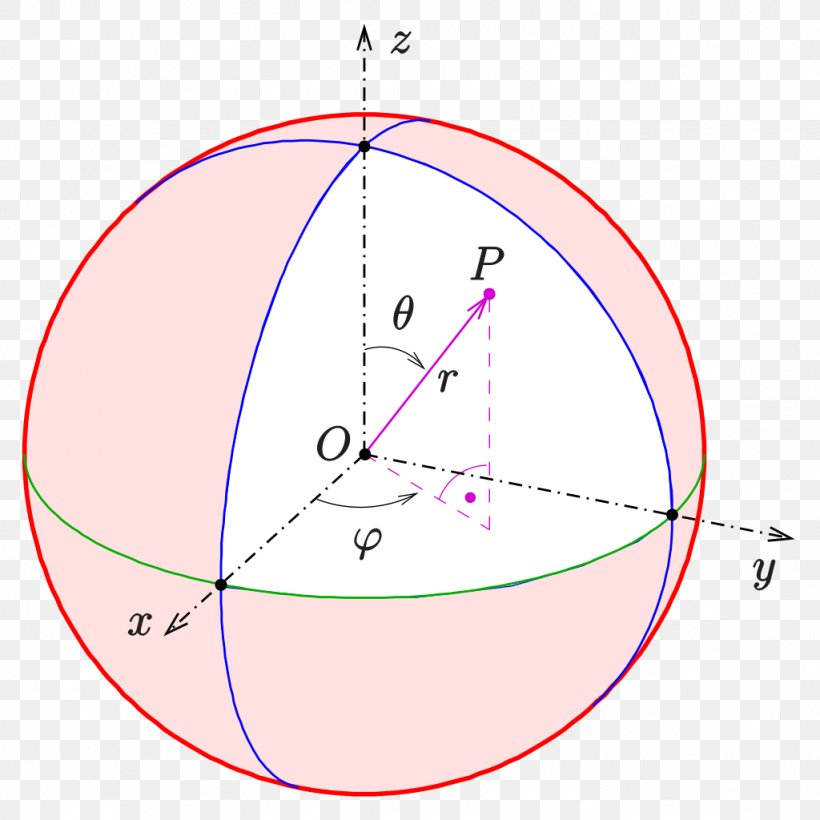
\includegraphics[width=\textwidth]{球坐标换元.png}
        \caption{球坐标换元}
        \label{fig:球坐标换元}
    \end{marginfigure}
        \begin{itemize}
            \item 雅可比行列式:$\frac{\partial(x,y,z)}{\partial(r,\theta,\varphi)}=r^2\cos(\varphi)$
            \item 参数范围:$(r,\theta,\varphi)\in(0,\infty)\times (-\pi,\pi)\times (-\frac{\pi}{2},\frac{\pi}{2})$
        \end{itemize}
\end{itemize}

\begin{kaobox}[frametitle=球坐标换元的说明]
    球坐标换元并不唯一,这里我们采用了\sidecite{于品}的定义,此外
    \[
        (x,y,z)=(r\cos(\varphi)\sin(\theta),r\sin(\varphi)\sin(\theta),r\cos(\theta))
    \]
    也是一个球坐标换元. 雅可比行列式为$r^2\sin(\theta)$. 参数取值范围为
    \[
        (r,\theta,\varphi)\in[0,\infty)\times[0,\pi)\times[0,2\pi)
    \]
\end{kaobox}

\subsection{Poisson公式和余面积公式}

球面外法向量:球面$(x-x_0)^2+(y-y_0)^2+(z-z_0)^2=r^2$在其上任意一点$(x,y,z)$的单位外法向量为
\[
    \left(\frac{x-x_0}{r},\frac{y-y_0}{r},\frac{z-z_0}{r}\right)
\]
\begin{theorem}[余面积公式]\label{thm:residual-area-formula}\marginnote{该公式串联了重积分、曲线积分、曲面积分,非常好用.}
    \begin{enumerate}
        \item \[\iint\limits_{r_1 \leqslant F(x, y) \leqslant r_2} f(x, y) \mathrm{d} x \mathrm{d} y=\int_{r_1}^{r_2} \mathrm{d} r \int_{F(x, y)=r} \frac{f(x, y)}{\sqrt{\left|\frac{\partial F}{\partial x}\right|^2+\left|\frac{\partial F}{\partial y}\right|^2}} \mathrm{d} s .\]
        \item \[\iiint\limits_{r_1 \leqslant F(x, y, z) \leqslant r_2} f(x, y, z) \mathrm{d} x \mathrm{d} y \mathrm{d} z=\int_{r_1}^{r_2} \mathrm{d} r \iint\limits_{F(x, y, z)=r} \frac{f(x, y, z)}{\sqrt{\left|\frac{\partial F}{\partial x}\right|^2+\left|\frac{\partial F}{\partial y}\right|^2+\left|\frac{\partial F}{\partial z}\right|^2}} \mathrm{d} S .\]
    \end{enumerate}
\end{theorem}

接下来展示一个利用余面积公式计算变态重积分的例子.

\begin{exercise}
计算
$$
\iiint\limits_{\Omega} \frac{1}{(1+x+y+z)^3} \mathrm{d} x \mathrm{d} y \mathrm{d} z,
$$
这里
$$
\Omega=\left\{(x, y, z) \in \mathbb{R}^3: x, y, z \geqslant 0, x+y+z \leqslant 1\right\} .
$$
\end{exercise}

\begin{solution}
    利用余面积公式\ref{thm:residual-area-formula},我们有
{\small
$$
\begin{aligned}
& \iiint\limits_{\Omega} \frac{1}{(1+x+y+z)^3} \mathrm{d} x \mathrm{d} y \mathrm{d} z=\iiint\limits_{x+y+z \leqslant 1} \frac{\chi_{[0,+\infty)^3}(x, y, z)}{(1+x+y+z)^3} \mathrm{d} x \mathrm{d} y \mathrm{d} z \\
& \quad=\frac{1}{\sqrt{3}} \int_{-\infty}^1 \mathrm{d} r \iint\limits_{x+y+z=r} \frac{\chi_{[0,+\infty)^3}(x, y, z)}{(1+x+y+z)^3} \mathrm{d} S=\frac{1}{\sqrt{3}} \int_0^1 \mathrm{d} r \iint\limits_{x+y+z=r} \frac{\chi_{[0,+\infty)^3}(x, y, z)}{(1+r)^3} \mathrm{d} S \\
& \quad=\frac{1}{\sqrt{3}} \int_0^1 \frac{1}{(1+r)^3} \mathrm{d} r \iint\limits_{x+y+z=r, x, y, z \geqslant 0} 1 \mathrm{d} S=\frac{1}{2} \int_0^1 \frac{r^2}{(1+r)^3} \mathrm{d} r=\frac{\ln 2}{2}-\frac{5}{16} .
\end{aligned}
$$
}
\end{solution}

作为多元积分换元法的应用,我们有Poisson公式\sidenote[][-1mm]{Poisson公式本质上依赖于还原法,所以实际运用中要注意变通,并不仅仅适用于上述形式. 此外Poisson公式在一些常见例题中,右端项还可以进一步简化为单变量积分,那样不利于记忆,这里给出便于记忆的形式. 而且,Poisson公式对于$n$重积分和$n$重曲面积分也是正确的.}.

\begin{theorem}[二元函数Poisson公式]
    设 $r>0, a, b, c \in \mathbb{R}$, 且下述积分有意义, 则有
{\small
\begin{align}
    \iint\limits_{x^2+y^2 \leqslant r^2} f(a x+b y) g\left(x^2+y^2\right) \mathrm{d} x \mathrm{d} y & =\iint\limits_{x^2+y^2 \leqslant r^2} f\left(\sqrt{a^2+b^2} y\right) g\left(x^2+y^2\right) \mathrm{d} x \mathrm{d} y \\
    \oint\limits_{x^2+y^2=r^2} f(a x+b y) g\left(x^2+y^2\right) \mathrm{d} s & =\oint\limits_{x^2+y^2=r^2} f\left(\sqrt{a^2+b^2} y\right) g\left(x^2+y^2\right) \mathrm{d} s .
\end{align}
}
\end{theorem}

\begin{theorem}[三元函数Poisson公式]
    设 $r>0, a, b, c \in \mathbb{R}$, 且下述积分有意义, 则有
{\small 
\begin{equation}
    \begin{split}
        & \iiint\limits_{x^2+y^2+z^2 \leqslant r^2}  f(a x+b y+c z) g\left(x^2+y^2+z^2\right) \mathrm{d} x \mathrm{d} y \mathrm{d} z \\
        = & \iiint\limits_{x^2+y^2+z^2 \leqslant r^2} f\left(\sqrt{a^2+b^2+c^2} z\right) g\left(x^2+y^2+z^2\right) \mathrm{d} x \mathrm{d} y \mathrm{d} z 
    \end{split}
\end{equation}
\begin{equation}
    \begin{split}
        & \iint\limits_{x^2+y^2+z^2=r^2}  f(a x+b y+c z) g\left(x^2+y^2+z^2\right) \mathrm{d} S \\
        = & \iint\limits_{x^2+y^2+z^2=r^2} f\left(\sqrt{a^2+b^2+c^2} z\right) g\left(x^2+y^2+z^2\right) \mathrm{d} S
    \end{split}
\end{equation}
}   
\end{theorem}

\begin{exercise}
    设$a,b,c\in\mathbb{R}\setminus\{0\}$,计算
    \[
        \iiint\limits_{x^2+y^2+z^2\leq r^2} (x^2+y^2+z^2)^p\left|ax+by+cz\right|^q\mathrm{d}x\mathrm{d}y\mathrm{d}z
    \]\marginnote{如何判断广义重积分的收敛性?直接加上绝对值爆算,算出来收敛就收敛,算出来发散就发散.}
\end{exercise}

\begin{solution}
    直接计算有
    \begin{align*}
        &\iiint\limits_{x^2+y^2+z^2\leq r^2} (x^2+y^2+z^2)^p\left|ax+by+cz\right|^q\mathrm{d}x\mathrm{d}y\mathrm{d}z\\
        &\overset{\text{余面积公式}\ref{thm:residual-area-formula}}{=}\int_0^r t^{2p}\mathrm{d}t\iint\limits_{x^2+y^2+z^2=t^2} (x^2+y^2+z^2)^p\left|ax+by+cz\right|^q\mathrm{d}S\\
        &\overset{\text{Poisson公式}\ref{thm:second-type-surface-integral-change-of-variable}}{=}(a^2+b^2+c^2)^{q/2}\int_0^r t^{2p}\mathrm{d}t\iint\limits_{x^2+y^2+z^2=t^2} \left|z\right|^q\mathrm{d}S\\
        &=2(a^2+b^2+c^2)^{q/2}\int_0^r t^{2p}\mathrm{d}t\iint\limits_{x^2+y^2+z^2=t^2,z\ge 0} z^q\mathrm{d}S\\
        &\overset{\text{换元法}}{=}2(a^2+b^2+c^2)^{q/2}\int_0^r t^{2p+q+2}\mathrm{d}t\iint\limits_{x^2+y^2+z^2=1,z\ge 0} z^q\mathrm{d}S\\
        &=2(a^2+b^2+c^2)^{q/2}\int_0^r t^{2p+q+2}\mathrm{d}t\iint\limits_{x^2+y^2\le 1} (1-x^2-y^2)^{(q-1)/2}\mathrm{d}x\mathrm{d}y\\
        &\overset{\text{余面积公式}\ref{thm:residual-area-formula}}{=}2(a^2+b^2+c^2)^{q/2}\int_0^r t^{2p+q+2}\mathrm{d}t\int_0^1\mathrm{d}v\int_{x^2+y^2=v^2} (1-x^2-y^2)^{(q-1)/2}\mathrm{d}s\\
        &=4\pi(a^2+b^2+c^2)^{q/2}\int_0^r t^{2p+q+2}\mathrm{d}t\int_0^1 v(1-v^2)^{(q-1)/2}\mathrm{d}v\\
    \end{align*}
    因此积分收敛等价于
    \[
    2p+q+2>-1,\quad \frac{q-1}{2}>-1
    \]
    于是积分收敛时,有
    \[
    \iiint\limits_{x^2+y^2+z^2\leq r^2} (x^2+y^2+z^2)^p\left|ax+by+cz\right|^q\mathrm{d}x\mathrm{d}y\mathrm{d}z=\frac{4\pi}{2p+q+3}(a^2+b^2+c^2)^{q/2}r^{2p+q+3}(q+1)
    \]
\end{solution}

\begin{exercise}
    计算积分
    \[
        L=\iiint_{(T)}\left(\frac{x^2}{a^2}+\frac{y^2}{b^2}+\frac{z^2}{c^2}\right) \mathrm{d}x\mathrm{d}y\mathrm{d}z
    \]
    其中$(T)$是整个椭球体$\frac{x^2}{a^2}+\frac{y^2}{b^2}+\frac{z^2}{c^2} \leqslant 1$.
\end{exercise}

\begin{solution}
    应用投影法,得
    \[
        L=\int_{-a}^a \frac{x^2}{a^2} \mathrm{d}x \iint_{(P_x)} \mathrm{d}y\mathrm{d}z+\int_{-b}^b \frac{y^2}{b^2} \mathrm{d}y \iint_{(Q_y)} \mathrm{d}z\mathrm{d}x+\int_{-c}^c \frac{z^2}{c^2} \mathrm{d}z \iint_{(R_z)} \mathrm{d}x\mathrm{d}y
    \]
    于是,
    \begin{align*}
        L &= \frac{\pi bc}{a^2} \int_{-a}^a x^2\left(1-\frac{x^2}{a^2}\right) \mathrm{d}x+\frac{\pi ca}{b^2} \int_{-b}^b y^2\left(1-\frac{y^2}{b^2}\right) \mathrm{d}y \\
        &\quad +\frac{\pi ab}{c^2} \int_{-c}^c z^2\left(1-\frac{z^2}{c^2}\right) \mathrm{d}z \\
        &= \frac{4}{5} \cdot \pi abc
    \end{align*}
\end{solution}


\section{投影法}

用于计算第二型曲面积分. 第二型曲面积分不同于第一型,它是有向的. 如下等式揭示了这两者的关系:
\[
    \iint_S Pdxdy+Qdydz+Rdzdx=\iint_S P\cos\alpha+Q\cos\beta+R\cos\gamma\mathrm{d}S
\]
其中$(\cos\alpha,\cos\beta,\cos\gamma)$是曲面$S$在点$(x,y,z)$处的法向量的方向余弦,给出了曲面$S$的那一侧.

根据上述讨论,我们已经可以将第二型曲面积分转化为第一型曲面积分,不过下面的定理(投影法)表明,可以直接把第二型曲面积分化为二重积分进行计算.
\begin{theorem}[投影法]
    设$R(x,y,z)$在光滑曲面
    $$
    S:z=z(x,y), (x,y)\in D
    $$
    上连续,则
    $$
    \iint_S R(x,y,z)dxdy=\pm \iint_D R(x,y,z(x,y))dxdy
    $$
    其中$S$表示上侧时取正号,$S$表示下侧时取负号.
\end{theorem}

\section{重积分换元技巧}

换元并不一定是标准换元,换元技巧是多样的.

\begin{exercise}
    计算曲面
    \[
        \left(\frac{x}{a}\right)^{2/3}+\left(\frac{y}{b}\right)^{2/3}+\left(\frac{z}{c}\right)^{2/3}=1
    \]
    所围立体的体积.
\end{exercise}

\begin{solution}
    按下面公式引入新的坐标:
    $$
    \begin{aligned}
    x= & a r \sin ^3 \varphi \cos ^3 \theta, y=b r \sin ^3 \varphi \sin ^3 \theta, z=c r \cos ^3 \varphi \\
    & (0 \leqslant r \leqslant 1,0 \leqslant \varphi \leqslant \pi, 0 \leqslant \theta \leqslant 2 \pi)
    \end{aligned}
    $$
    这时雅可比式
    $$
    J=9 a b c r^2 \sin ^5 \varphi \cos ^2 \varphi \sin ^2 \theta \cos ^2 \theta,
    $$
    所以

    $$
    V=9 a b c \int_0^1 r^2 d r \int_0^\pi \sin ^5 \varphi \cos ^2 \varphi d \varphi \int_0^{2 \pi} \sin ^2 \theta \cos ^2 \theta d \theta=\frac{4}{35} \pi a b c .
    $$
\end{solution}

\begin{exercise}
    求曲面
    \[
        (x+y+z)^2=a y, x=0, y=0, z=0
    \]
    所围立体的体积.
\end{exercise}

\begin{solution}
    令
    $$
    \begin{aligned}
    x= & r \sin ^2 \varphi \cos ^2 \theta, y=r \sin ^2 \varphi \sin ^2 \theta, z=r \cos ^2 \varphi \\
    & \left(r \geqslant 0,0 \leqslant \varphi \leqslant \frac{\pi}{2}, 0 \leqslant \theta \leqslant \frac{\pi}{2}\right)
    \end{aligned}
    $$
    这时雅可比式
    $$
    J=4 r^2 \sin ^3 \varphi \cos \varphi \sin \theta \cos \theta
    $$
    代入原方程$(x+y+z)^2=ay$得:
    $$
    (r\sin^2\varphi\cos^2\theta + r\sin^2\varphi\sin^2\theta + r\cos^2\varphi)^2 = ar\sin^2\varphi\sin^2\theta
    $$
    即
    $$
    r^2 = ar\sin^2\varphi\sin^2\theta
    $$
    所以$r = a\sin^2\varphi\sin^2\theta$,因此体积为$V = \frac{a^3}{60}$.
\end{solution}

\begin{exercise}
    计算逐次积分
    $$
    \int_1^{\infty} d z \int_1^{\infty} y d y \int_0^{\frac{1}{y z}} e^{x y z} x^2 d x
    $$
\end{exercise}

\begin{solution}
    将它换作三重积分
    $$
    \iiint_{\substack{x \geqslant 0, y, z \geqslant 1 \\ x y z \leqslant 1}} e^{x y z} x^2 y d x d y d z,
    $$
    再采用替换
    $$
    x=u, \quad y=\frac{u+v}{u}, \quad z=\frac{u+v+w}{u+v}, \quad J=\frac{1}{u(u+v)} .
    $$
    积分化为:
    $$
    \iiint_{\substack{u, v, w \geqslant 0 \\ u+v+w \leqslant 1}} e^{u+v+w} d u d v d w
    $$
    这很容易计算,结果为$\frac{e}{2}-1$.
\end{solution}

\begin{exercise}
    计算积分
    $$
    H=\iiint_{\substack{x, y, z \geqslant 0 \\ x^2+y^2+z^2 \leqslant R^2}} \frac{x y z d x d y d z}{\sqrt{\alpha^2 x^2+\beta^2 y^2+\gamma^2 z^2}} \quad(\alpha>\beta>\gamma>0)
    $$
\end{exercise}

\begin{solution}
    在球坐标下
    $$
    H=\int_0^{\frac{\pi}{2}} \int_0^{\frac{\pi}{2}} \int_0^R \frac{r^4 \sin ^3 \varphi \cos \varphi \sin \theta \cos \theta d r d \varphi d \theta}{\sqrt{\alpha^2 \sin ^2 \varphi \cos ^2 \theta+\beta^2 \sin ^2 \varphi \sin ^2 \theta+\gamma^2 \cos ^2 \varphi}} .
    $$
    进行替换 $\sin ^2 \varphi=u, \sin ^2 \theta=v$ 较为方便. 则
    $$
    \begin{aligned}
    H & =\frac{1}{4} \int_0^1 \int_0^1 \int_0^R r^4 \frac{u d r d u d v}{\sqrt{\alpha^2 u(1-v)+\beta^2 u v+\gamma^2(1-u)}} \\
    & =\frac{R^5}{20} \int_0^1 u d u \int_0^1 \frac{d v}{\sqrt{\left[\gamma^2+\left(\alpha^2-\gamma^2\right) u\right]+\left(\beta^2-\alpha^2\right) u v}} \\
    & =\frac{R^5}{15} \frac{\beta \gamma+\gamma \alpha+\alpha \beta}{(\beta+\gamma)(\gamma+\alpha)(\alpha+\beta)} .
    \end{aligned}
    $$
\end{solution}

\section{三角函数积分}

计算:
\[
    \int_0^{\pi/2}\sin^n x dx=\begin{cases}
        \frac{(n-1)!!}{n!!}\cdot\frac{\pi}{2},&n\text{为偶数}\\
        \frac{(n-1)!!}{n!!},&n\text{为奇数}
    \end{cases}
\]
\begin{solution}
    令$I_n=\int_0^{\pi/2}\sin^n x dx$,则有
    \begin{align*}
        I_n &= \int_0^{\pi/2}\sin^n x dx = \int_0^{\pi/2}\sin^{n-1} x \sin x dx \\
        &= \int_0^{\pi/2}\sin^{n-1} x d(\cos x) \\
        &= -\cos x \sin^{n-1} x \Big|_0^{\pi/2} + (n-1)\int_0^{\pi/2}\sin^{n-2} x (1-\cos^2 x) dx \\
        &= (n-1)I_{n-2}-(n-1)I_n
    \end{align*}
    于是
    \[
        I_n=\frac{n-1}{n}I_{n-2},\quad I_0=\frac{\pi}{2},I_1=1
    \]
    递推下去,当$n$为偶数时,$I_n = \frac{(n-1)!!}{n!!}\cdot\frac{\pi}{2}$,当$n$为奇数时,$I_n = \frac{(n-1)!!}{n!!}$.
\end{solution}

\section{特殊函数}

\begin{definition}[Gamma函数]
    Gamma函数定义为
    $$
    \Gamma(x) = \int_0^\infty t^{x-1}e^{-t}\mathrm{d}t
    $$
\end{definition}

\begin{theorem}[Gamma函数的性质]
    Gamma函数满足以下性质:
    \begin{enumerate}
        \item $\Gamma(x+1) = x\Gamma(x)$
        \item $\Gamma(n) = (n-1)!,\forall n\in\mathbb{N}$
        \item $\Gamma\left(\frac{1}{2}\right) = \sqrt{\pi}$
        \item $\Gamma(x)\Gamma(1-x) = \frac{\pi}{\sin(x\pi)},\forall x\in(0,1)$\sidenote{余元公式.}
    \end{enumerate}
\end{theorem}

\begin{definition}[Beta函数]
    Beta函数定义为
    $$
    B(x,y) = \int_0^1 t^{x-1}(1-t)^{y-1}\mathrm{d}t=\frac{\Gamma(x)\Gamma(y)}{\Gamma(x+y)}
    $$
\end{definition}

\begin{theorem}[Beta函数的性质]
    Beta函数满足以下性质:
    \begin{enumerate}
        \item $B(x,y) = B(y,x)$
        \item $B(x,y) = \int_0^\infty \frac{u^{x-1}}{(1+u)^{x+y}}\mathrm{d}u$\sidenote{换元令$t=\frac{u}{1+u}$即可得到}
        \item $B(x,y) = \frac{\Gamma(x)\Gamma(y)}{\Gamma(x+y)}$
        \item $B(x,1-x) = \frac{\pi}{\sin(x\pi)},\forall x\in(0,1)$\sidenote{余元公式.}
        \item $B(x,y)={\color{red}2}\int_0^{\pi/2}\sin^{2x-1}\theta\cos^{2y-1}\theta\mathrm{d}\theta$\sidenote{令$t=\sin^2\theta$换元.}
        \item $B\left(\frac{1}{2},\frac{1}{2}\right) = \pi$
    \end{enumerate}
\end{theorem}

\begin{exercise}
    证明: 对任意 $p>0$ 都有
$$
\int_0^{\frac{\pi}{2}} \sin ^p x \mathrm{~d} x=\int_0^{\frac{\pi}{2}} \cos ^p x \mathrm{~d} x=\frac{1}{2} \mathrm{~B}\left(\frac{1}{2}, \frac{p+1}{2}\right) .
$$
并据此计算当 $p$ 为正整数时的积分值.
\end{exercise}
\begin{exercise}
    证明: $\lim _{n \rightarrow \infty} \int_0^{+\infty} \mathrm{e}^{-x^n} \mathrm{~d} x=1$.
\end{exercise}

\section{曲线积分与曲面积分}

设曲面 $S$ 的参数方程为
$$
x=x(u, v), \quad y=y(u, v), \quad z=z(u, v), \quad(u, v) \in D,
$$
其中, $D$ 是平面上一个具有连续边界的有界闭区域, $x(u, v), y(u, v)$ 和 $z(u, v)$ 都是区域 $D$ 上的连续可微函数, 使得矩阵
$$
\left(\begin{array}{lll}
x_u & y_u & z_u \\
x_v & y_v & z_v
\end{array}\right)
$$
在 $D$ 上每个点处的秩都是 2 . 又设 $f(x, y, z)$ 是定义在曲面 $S$ 上的连续函数. 则 $f$ 在 $S$ 上可积, 且
\begin{align*}
\iint f(x, y, z) \mathrm{d} \sigma &= \iint f(x(u, v), y(u, v), z(u, v)) \\
&\quad \times \sqrt{\left|\frac{\partial(x, y)}{\partial(u, v)}\right|^2+\left|\frac{\partial(y, z)}{\partial(u, v)}\right|^2+\left|\frac{\partial(z, x)}{\partial(u, v)}\right|^2} \mathrm{~d} u \mathrm{~d} v
\end{align*}

\begin{theorem}[第二型曲线积分与第一型曲线积分的关系]
    设 $C$ 是连续可微的有向曲线, 它在其上点 $(x, y, z)$ 处的单位切向量为 $\boldsymbol{v}(x, y, z)$. 又设 $\boldsymbol{F}(x, y, z)$ 是定义在曲线 $C$ 上的向量函数. 则有
    $$
    \int_C \boldsymbol{F}(x, y, z) \cdot \mathrm{d} \boldsymbol{r}=\int_C \boldsymbol{F}(x, y, z) \cdot \boldsymbol{v}(x, y, z) \mathrm{d} s .
    $$
    即 $\boldsymbol{F}(x, y, z)$ 沿曲线 $C$ 的第二型曲线积分等于它与 $C$ 的单位切向量函数 $\boldsymbol{v}(x, y, z)$ 的内积 $\boldsymbol{F}(x, y, z) \cdot \boldsymbol{v}(x, y, z)$ 在 $C$ 上的第一型曲线积分.
\end{theorem}

\begin{theorem}[第二型曲面积分与第一型曲面积分的关系]
    设有向曲面 $S$ 的参数方程为
    $$
    x=x(u, v), \quad y=y(u, v), \quad z=z(u, v), \quad(u, v) \in D,
    $$
    其中, $D$ 是平面上一个具有连续边界的有界闭区域, $x(u, v), y(u, v)$ 和 $z(u, v)$ 都是区域 $D$ 上的连续可微函数, 使得矩阵
    $$
    \left(\begin{array}{lll}
    x_u & y_u & z_u \\
    x_v & y_v & z_v
    \end{array}\right)
    $$
    在 $D$ 上每个点处的秩都是 2. 又设 $\boldsymbol{F}(x,y,z)$ 是定义在曲面 $S$ 上的向量函数. 则有
    $$
    \iint_S \boldsymbol{F}(x,y,z) \cdot \mathrm{d}\boldsymbol{S} = \iint_S \boldsymbol{F}(x,y,z) \cdot \boldsymbol{n}(x,y,z) \mathrm{d}\sigma,
    $$
    其中 $\boldsymbol{n}(x,y,z)$ 是曲面 $S$ 在点 $(x,y,z)$ 处的单位法向量.
\end{theorem}

\begin{theorem}[第二型曲面积分正负号的确定]\label{第二型曲面积分正负号的确定}
    设有向曲面 $S$ 的参数方程为
    $$
    x=x(u, v), \quad y=y(u, v), \quad z=z(u, v), \quad(u, v) \in D,
    $$
    其中, $D$ 是平面上一个具有连续边界的有界闭区域, $x(u, v), y(u, v)$ 和 $z(u, v)$ 都是区域 $D$ 上的连续可微函数, 使得矩阵
    $$
    \left(\begin{array}{lll}
    x_u & y_u & z_u \\
    x_v & y_v & z_v
    \end{array}\right)
    $$
    在 $D$ 上每个点处的秩都是 2. 又设 $\boldsymbol{F}(x, y, z)$ 是定义在曲面 $S$ 上的连续向量函数, 其分量表达式为
    $$
    \boldsymbol{F}(x, y, z)=P(x, y, z) \boldsymbol{i}+Q(x, y, z) \boldsymbol{j}+R(x, y, z) \boldsymbol{k} .
    $$
    则有
    $$
    \iint_S \boldsymbol{F}(x,y,z) \cdot \mathrm{d}\boldsymbol{S} = \iint_D \left|\begin{array}{ccc}
    P & Q & R \\
    x_u & y_u & z_u \\
    x_v & y_v & z_v
    \end{array}\right| \mathrm{d}u\mathrm{d}v.
    $$
    其中, $P(u, v)=P(x(u, v), y(u, v), z(u, v)), Q(u, v)=Q(x(u, v), y(u, v), z(u, v))$,$ R(u, v)=R(x(u, v), y(u, v), z(u, v))$. 等式右端正负号的选取规则为当 $S$ 的给定法向量 $\boldsymbol{n}$ 与向量 $\boldsymbol{r}_u \times \boldsymbol{r}_v$ (其中 $\boldsymbol{r}=x(u, v) \boldsymbol{i}+y(u, v) \boldsymbol{j}+z(u, v) \boldsymbol{k}$) 同向时取正号, 反向时则取负号.
\end{theorem}

设有向曲面 $S$ 的参数方程为
$$
x=x(u, v), \quad y=y(u, v), \quad z=z(u, v), \quad(u, v) \in D,
$$
其中, $D$ 是平面上一个具有连续边界的有界闭区域, $x(u, v), y(u, v)$ 和 $z(u, v)$ 都是区域 $D$ 上的连续可微函数, 使得矩阵
$$
\left(\begin{array}{lll}
x_u & y_u & z_u \\
x_v & y_v & z_v
\end{array}\right)
$$
在 $D$ 上每个点处的秩都是 2 . 又设 $f(x, y, z)$ 是定义在曲面 $S$ 上的连续函数. 则有
$$
\begin{aligned}
& \iint_S f(x, y, z) \mathrm{d} y \mathrm{~d} z= \pm \iint_D f(x(u, v), y(u, v), z(u, v)) \frac{\partial(y, z)}{\partial(u, v)} \mathrm{d} u \mathrm{~d} v \\
& \iint_S f(x, y, z) \mathrm{d} z \mathrm{~d} x= \pm \iint_D f(x(u, v), y(u, v), z(u, v)) \frac{\partial(z, x)}{\partial(u, v)} \mathrm{d} u \mathrm{~d} v \\
& \iint_S f(x, y, z) \mathrm{d} x \mathrm{~d} y= \pm \iint_D f(x(u, v), y(u, v), z(u, v)) \frac{\partial(x, y)}{\partial(u, v)} \mathrm{d} u \mathrm{~d} v .
\end{aligned}
$$
这里正负号的选取规则如定理\ref{第二型曲面积分正负号的确定}所述.

特别地,如果曲面 $S$ 是由显式方程
$$
z=\varphi(x, y), \quad(x, y) \in D
$$
给出,其中, $D$ 是平面上具连续边界的有界闭区域, $f(x, y)$ 是定义在区域 $D$ 上的一阶连续可微函数,且 $S$ 的正向指向曲面的上方,则应用以上公式可知
$$
\begin{aligned}
& \iint_S f(x, y, z) \mathrm{d} y \mathrm{~d} z=-\iint_D f(x, y, \varphi(x, y)) \varphi_x(x, y) \mathrm{d} x \mathrm{~d} y \\
& \iint_S f(x, y, z) \mathrm{d} z \mathrm{~d} x=-\iint_D f(x, y, \varphi(x, y)) \varphi_y(x, y) \mathrm{d} x \mathrm{~d} y \\
& \iint_S f(x, y, z) \mathrm{d} x \mathrm{~d} y=\iint_D f(x, y, \varphi(x, y)) \mathrm{d} x \mathrm{~d} y
\end{aligned}
$$
与第二型曲线积分类似,对于第二型曲面积分,改变曲面的定向就改变了积分的正负号,即
$$
\begin{aligned}
& \iint_{S^{-}} P(x, y, z) \mathrm{d} y \mathrm{~d} z+Q(x, y, z) \mathrm{d} z \mathrm{~d} x+R(x, y, z) \mathrm{d} x \mathrm{~d} y \\
= & -\iint_S P(x, y, z) \mathrm{d} y \mathrm{~d} z+Q(x, y, z) \mathrm{d} z \mathrm{~d} x+R(x, y, z) \mathrm{d} x \mathrm{~d} y,
\end{aligned}
$$
其中 $S^{-}$表示把 $S$ 的方向改变为反方向所得到的有向曲面。这是第二型曲面积分与第一型曲面积分的一个重要区别。
\begin{example}
计算第二型曲面积分
$$
I=\iint_S \frac{\mathrm{~d} y \mathrm{~d} z}{x}+\frac{\mathrm{d} z \mathrm{~d} x}{y}+\frac{\mathrm{d} x \mathrm{~d} y}{z},
$$
其中 $S$ 是椭球面 $\frac{x^2}{a^2}+\frac{y^2}{b^2}+\frac{z^2}{c^2}=1$, 以外侧为正侧.
\end{example}

\begin{solution}
    利用对称性,只需计算三个积分中的任何一个. 下面以第三个积分 $I_3$ 为例来计算。椭球面 $S$ 分为上、下两半,分别记为 $S_1$ 和 $S_2$ 。因为 $S_1$ 以上侧为正向, $S_2$ 以下侧为正向,所以
$$
\begin{aligned}
I_3 & =\iint_{S_1} \frac{\mathrm{~d} x \mathrm{~d} y}{z}+\iint_{S_2} \frac{\mathrm{~d} x \mathrm{~d} y}{z} \\
& =\iint_D \frac{\mathrm{~d} x \mathrm{~d} y}{c \sqrt{1-\frac{x^2}{a^2}-\frac{y^2}{b^2}}}-\iint_D \frac{\mathrm{~d} x \mathrm{~d} y}{-c \sqrt{1-\frac{x^2}{a^2}-\frac{y^2}{b^2}}}=\frac{2}{c} \iint_D \frac{\mathrm{~d} x \mathrm{~d} y}{\sqrt{1-\frac{x^2}{a^2}-\frac{y^2}{b^2}}},
\end{aligned}
$$
其中 $D$ 是平面上的椭圆形区域 $\frac{x^2}{a^2}+\frac{y^2}{b^2} \leqslant 1$. 作广义极坐标变换 $x=\operatorname{ar} \cos \theta, y=$ $b r \sin \theta$ ,便有
$$
I_3=\frac{2}{c} \int_0^{2 \pi} \int_0^1 \frac{a b r}{\sqrt{1-r^2}} \mathrm{~d} r \mathrm{~d} \theta=\left.\frac{4 \pi a b}{c}\left(-\sqrt{1-r^2}\right)\right|_0 ^1=\frac{4 \pi a b}{c} .
$$
由对称性有
$$
I_1=\frac{4 \pi b c}{a}, \quad I_2=\frac{4 \pi a c}{b}
$$
因此
$$
I=I_1+I_2+I_3=\frac{4 \pi}{a b c}\left(a^2 b^2+a^2 c^2+b^2 c^2\right) .
$$
\end{solution}

\section{各种积分之间的联系与场论初步}

参考\cite{邓东皋},\cite{崔尚斌}.

\subsection{格林公式}
\begin{theorem}[\textcolor{green}{格林公式}]\label{格林公式}
设 $D$ 是由逐段光滑闭曲线 $L$ 围成的平面单连通闭区域, 函数 $P(x, y), Q(x, y)$ 在 $D$ 上有一阶连续偏导数, 则有
$$
\iint_D\left(\frac{\partial Q}{\partial x}-\frac{\partial P}{\partial y}\right) \mathrm{d} x \mathrm{~d} y=\oint_L P \mathrm{d} x+Q \mathrm{~d} y .
$$
其中右端的积分路径是闭曲线 $L$, 方向取正向.
\end{theorem}
\begin{marginfigure}
    \centering
    \includegraphics[width=\textwidth]{Green.png}
    \caption{格林公式}
    \label{fig:格林公式}
\end{marginfigure}
回忆闭曲线正向的含义是,当一人沿着曲线 $L$ 走时,区域 $D$ 始终在他的左边.

格林公式\ref{格林公式}还可以用来计算曲线所围成区域的面积,公式如下
\[
|D|=\frac{1}{2}\oint_L x \mathrm{d} y-y \mathrm{d} x
\]
如果使用极坐标换元,则有
\[
|D|=\frac{1}{2}\oint_L r^2 \mathrm{d} \theta 
\]
\marginnote[*-1]{注意这里的$\theta$取值范围要根据实际情况而定,并不是简单的从$0$到$2\pi$}

\begin{corollary}[二维分部积分公式]
    设 $D$ 是平面上由一条或数条分段光滑的闭曲线围成的区域, $P, Q, U, V$ 是 $D$ 上的连续可微函数. 则有
$$
\iint_D\left(P \frac{\partial U}{\partial x}+Q \frac{\partial V}{\partial y}\right) \mathrm{d} x \mathrm{~d} y=\int_{\partial D} P U \mathrm{~d} y-Q V \mathrm{~d} x-\iint_D\left(U \frac{\partial P}{\partial x}+V \frac{\partial Q}{\partial y}\right) \mathrm{d} x \mathrm{~d} y .
$$
其中 $\partial D$ 的正向取为按 $D$ 右旋的方向.
\end{corollary}
\begin{proof}
    根据格林公式, 有 
    \begin{align*}
        & \iint_D\left(P \frac{\partial U}{\partial x}+Q \frac{\partial V}{\partial y}\right) \mathrm{d} x \mathrm{~d} y+\iint_D\left(U \frac{\partial P}{\partial x}+V \frac{\partial Q}{\partial y}\right) \mathrm{d} x \mathrm{~d} y \\
        = & \iint_D\left(\frac{\partial(P U)}{\partial x}+\frac{\partial(Q V)}{\partial y}\right) \mathrm{d} x \mathrm{~d} y=\int_{\partial D} P U \mathrm{~d} y-Q V \mathrm{~d} x .
    \end{align*}
\end{proof}

\begin{example}[计算曲线积分]\label{ex:格林公式}
    计算曲线积分
    $$
    I=\int_C \frac{x \mathrm{~d} y-y \mathrm{~d} x}{x^2+y^2}
    $$
    其中 $C$ 是逆时针旋转且不经过坐标原点的封闭分段光滑曲线. 考虑两种情况:
    \begin{enumerate}
        \item $C$ 包围的区域不包含坐标原点;
        \item $C$ 包围的区域包含坐标原点.
    \end{enumerate}
\end{example}

\begin{marginfigure}
    \centering
    \includegraphics[width=\textwidth]{Green_ex1.png}
    \caption{例\ref{ex:格林公式}中的$D / B_{\varepsilon}(0)$}
    \label{fig:格林公式ex1}
\end{marginfigure}

\begin{solution}
    用 $D$ 表小 $C$ 包围的区域. 则当 $D$ 不包含坐标原点时, 函数 $P(x, y)=-\frac{y}{x^2+y^2}$ 和 $Q(x, y)=\frac{x}{x^2+y^2}$ 都在 $D$ 中连续可微. 因此应用格林公式得
$$
\begin{aligned}
\int_C \frac{x \mathrm{~d} y-y \mathrm{~d} x}{x^2+y^2} & =\iint_D\left[\frac{\partial}{\partial x}\left(\frac{x}{x^2+y^2}\right)-\frac{\partial}{\partial y}\left(\frac{-y}{x^2+y^2}\right)\right] \mathrm{d} x \mathrm{~d} y \\
& =\iint_D\left(\frac{y^2-x^2}{\left(x^2+y^2\right)^2}+\frac{x^2-y^2}{\left(x^2+y^2\right)^2}\right) \mathrm{d} x \mathrm{~d} y=0 .
\end{aligned}
$$
当 $D$ 包含坐标原点时, 因原点是函数 $P(x, y)=-\frac{y}{x^2+y^2}$ 和 $Q(x, y)=\frac{x}{x^2+y^2}$ 的奇点, 即 $P$ 和 $Q$ 不可微因而不满足格林公式条件的点, 所以不能直接应用格林公式. 这时取 $\varepsilon>0$ 充分小使闭圆盘 $\overline{B_{\varepsilon}(0)}$ 包含于 $D^{\circ}$ (图 20-3-5). 在区域 $D \backslash B_{\varepsilon}(0)$ 上应用格林公式得
$$
\begin{aligned}
\int_C \frac{x \mathrm{~d} y-y \mathrm{~d} x}{x^2+y^2} & =\iint_{D \backslash B_{\varepsilon}(0)}\left[\frac{\partial}{\partial x}\left(\frac{x}{x^2+y^2}\right)-\frac{\partial}{\partial y}\left(\frac{-y}{x^2+y^2}\right)\right] \mathrm{d} x \mathrm{~d} y+\int_{\partial B_{\varepsilon}(0)} \frac{x \mathrm{~d} y-y \mathrm{~d} x}{x^2+y^2} \\
& =\frac{1}{\varepsilon^2} \int_{\partial B_{\varepsilon}(0)} x \mathrm{~d} y-y \mathrm{~d} x
\end{aligned}
$$
对最后这个积分再次应用格林公式,就得到
$$
\begin{aligned}
\int_C \frac{x \mathrm{~d} y-y \mathrm{~d} x}{x^2+y^2} & =\frac{1}{\varepsilon^2} \iint_{B_{\varepsilon}(0)}\left(\frac{\partial x}{\partial x}-\frac{\partial(-y)}{\partial y}\right) \mathrm{d} x \mathrm{~d} y \\
& =\frac{2}{\varepsilon^2} \iint_{B_{\varepsilon}(0)} \mathrm{d} x \mathrm{~d} y=\frac{2}{\varepsilon^2} \cdot \pi \varepsilon^2=2 \pi
\end{aligned}
$$
\end{solution}



\subsection{高斯公式}
\begin{theorem}[高斯公式]\label{thm:gauss}
设空间区域 $V$ 由分片光滑的双侧封闭曲面 $S$ 围成,函数 $P(x, y, z), Q(x, y, z), R(x, y, z)$ 在 $V$ 及 $S$ 上有一阶连续偏导数, 则有
$$
\iiint_V\left(\frac{\partial P}{\partial x}+\frac{\partial Q}{\partial y}+\frac{\partial R}{\partial z}\right) \mathrm{d} x \mathrm{~d} y \mathrm{~d} z=\oiint_S P \mathrm{~d} y \mathrm{~d} z+Q \mathrm{~d} z \mathrm{~d} x+R \mathrm{~d} x \mathrm{~d} y,
$$
其中 $S$ 的方向为外侧.
\end{theorem}
\begin{corollary}[三维分部积分公式]
    设 $\Omega$ 是 $\mathbf{R}^3$ 中具有连续边界的有界闭区域, $P, Q, R, U, V, W$ 都是 $\Omega$ 上的连续可微函数. 则有
$$
\begin{aligned}
& \iiint_{\Omega}\left(P \frac{\partial U}{\partial x}+Q \frac{\partial V}{\partial y}+R \frac{\partial W}{\partial z}\right) \mathrm{d} x \mathrm{~d} y \mathrm{~d} z\\
= & \iint_{\partial \Omega}(P U \cos \alpha+Q V \cos \beta+R W \cos \gamma) \mathrm{d} \sigma \\
& -\iiint_{\Omega}\left(U \frac{\partial P}{\partial x}+V \frac{\partial Q}{\partial y}+W \frac{\partial R}{\partial z}\right) \mathrm{d} x \mathrm{~d} y \mathrm{~d} z .
\end{aligned}
$$
其中 $(\cos \alpha, \cos \beta, \cos \gamma)$ 是 $\Omega$ 边界的单位外法向量的方向余弦.
\end{corollary}
\begin{proof}
    应用高斯公式, 有
    {
        \small
        \begin{align*}
            & \iiint_{\Omega}\left(P \frac{\partial U}{\partial x}+Q \frac{\partial V}{\partial y}+R \frac{\partial W}{\partial z}\right) \mathrm{d} x \mathrm{~d} y \mathrm{~d} z+\iiint_{\Omega}\left(U \frac{\partial P}{\partial x}+V \frac{\partial Q}{\partial y}+W \frac{\partial R}{\partial z}\right) \mathrm{d} x \mathrm{~d} y \mathrm{~d} z \\
            = & \iiint_{\Omega}\left(\frac{\partial(P U)}{\partial x}+\frac{\partial(Q V)}{\partial y}+\frac{\partial(R W)}{\partial z}\right) \mathrm{d} x \mathrm{~d} y \mathrm{~d} z \\
            = & \iint_{\partial \Omega} P U \mathrm{~d} y \mathrm{~d} z+Q V \mathrm{~d} z \mathrm{~d} x+R W \mathrm{~d} x \mathrm{~d} y \\
            = & \iint_{\partial \Omega}(P U \cos \alpha+Q V \cos \beta+R W \cos \gamma) \mathrm{d} \sigma .
        \end{align*}
    }
\end{proof}

\subsection{斯托克斯公式}

\begin{theorem}[斯托克斯公式]
    若光滑曲面 $S$ 的边界为光滑曲线 $L$, 函数 $P, Q, R$ 在曲面 $S$ 及曲线 $L$ 上具有连续的一阶偏导数,则
    $$
    \begin{aligned}
    & \iint_S\left(\frac{\partial R}{\partial y}-\frac{\partial Q}{\partial z}\right) \mathrm{d} y \mathrm{~d} z+\left(\frac{\partial P}{\partial z}-\frac{\partial R}{\partial x}\right) \mathrm{d} z \mathrm{~d} x+\left(\frac{\partial Q}{\partial x}-\frac{\partial P}{\partial y}\right) \mathrm{d} x \mathrm{~d} y \\
    = & \oint_L P \mathrm{~d} x+Q \mathrm{~d} y+R \mathrm{~d} z
    \end{aligned}
    $$
    其中 $S$ 的侧与 $L$ 的方向按右手法则确定, 即若四个手指的方向为 $L$ 的方向,则大拇指所指的方向就是曲面 $S$ 的方向, 如图 22-13.
\end{theorem}

斯托克斯公式建立了函数在空间曲面 $S$ 上的第二型曲面积分与其 "原函数" 在 $S$ 的边界曲线 $L$ 上的第二型曲线积分之间的联系, 因此也是牛顿 - 莱布尼茨公式的一种高维的推广. 利用两种曲面积分之间的关系, 常把它写成如下便于记忆的形式:
$$
\begin{aligned}
\oint_L P \mathrm{~d} x+Q \mathrm{~d} y+R \mathrm{~d} z
& =\iint_S\left|\begin{array}{ccc}
\mathrm{d} y \mathrm{~d} z & \mathrm{~d} z \mathrm{~d} x & \mathrm{~d} x \mathrm{~d} y \\
\frac{\partial}{\partial x} & \frac{\partial}{\partial y} & \frac{\partial}{\partial z} \\
P & Q & R
\end{array}\right| \\
& =\iint_S\left|\begin{array}{ccc}
\cos \alpha & \cos \beta & \cos \gamma \\
\frac{\partial}{\partial x} & \frac{\partial}{\partial y} & \frac{\partial}{\partial z} \\
P & Q & R
\end{array}\right| \mathrm{d} S .
\end{aligned}
$$
不难看出,格林公式是斯托克斯公式的特殊情形。当 $L$ 是 $O x y$ 平面上的闭曲线时, $\mathrm{d} z=0$. 取 $S$ 为 $O x y$ 面上由 $L$ 围成的区域, 则 $S$ 在 $O_{y z}$ 和 $O_{z x}$ 平面上的投影为零, 因此对 $\mathrm{d} y \mathrm{~d} z, \mathrm{~d} z \mathrm{~d} x$ 的积分为 0 , 这时斯托克斯公式化为格林公式
$$
\oint_L P \mathrm{~d} x+Q \mathrm{~d} y=\iint_S\left|\begin{array}{cc}
\frac{\partial}{\partial x} & \frac{\partial}{\partial y} \\
P & Q
\end{array}\right| \mathrm{d} x \mathrm{~d} y .=\iint_S\left(\frac{\partial Q}{\partial x}-\frac{\partial P}{\partial y}\right) \mathrm{d} x \mathrm{~d} y .
$$

\begin{example}
    计算曲线积分
$$
\int_C\left(x^2-y z\right) \mathrm{d} x+\left(y^2-x z\right) \mathrm{d} y+\left(z^2-x y\right) \mathrm{d} z,
$$
其中 $C$ 是螺线 $x=a \cos \theta, y=a \sin \theta, z=b \theta$ 从点 $A(a, 0,0)$ 到点 $B(a, 0,2 \pi b)$ 的部分.
\end{example}

\begin{solution}
令 $S$ 是以由直线段 $A B$ 和曲线 $C$ 形成的封闭曲线为边界的任意光滑曲面,正侧为 $O z$ 轴的正向一侧. 则根据斯托克斯公式有
$$
\begin{aligned}
& \int_C\left(x^2-y z\right) \mathrm{d} x+\left(y^2-x z\right) \mathrm{d} y+\left(z^2-x y\right) \mathrm{d} z \\
& =\int_{\overline{A B}}\left(x^2-y z\right) \mathrm{d} x+\left(y^2-x z\right) \mathrm{d} y+\left(z^2-x y\right) \mathrm{d} z+\iint_S\left|\begin{array}{ccc}
\mathrm{d} y \mathrm{~d} z & \mathrm{~d} z \mathrm{~d} x & \mathrm{~d} x \mathrm{~d} y \\
\frac{\partial}{\partial x} & \frac{\partial}{\partial y} & \frac{\partial}{\partial z} \\
x^2-y z & y^2-x z & z^2-x y
\end{array}\right| \\
& =\int_0^{2 \pi b} z^2 \mathrm{~d} z=\frac{8}{3} \pi^3 b^3 .
\end{aligned}
$$
\end{solution}

\section{期末练习}

\begin{exercise}
    求 $\frac{\mathrm{d}}{\mathrm{d} x} \int_x^{x^2} \frac{\sin x y}{y} \mathrm{~d} y$, 其中 $x>0$.\marginnote{含参变量积分求导}
\end{exercise}
\begin{solution}
    利用\ref{thm:derivative-of-integral-with-parameter},我们有
    \begin{align*}
        ...=&\frac{2\sin x^3}{x^2}-\frac{\sin x^2}{x}+\int_x^{x^2}\cos(xy)\mathrm{d}y\\
        =&\frac{2\sin x^3}{x^2}-\frac{\sin x^2}{x}+\frac{\sin x^3}{x^2}-\frac{\sin x^2}{x}\\
        =&\frac{3\sin x^3}{x^2}-\frac{2\sin x^2}{x}
    \end{align*}
\end{solution}

\begin{exercise}
    利用Euler积分计算$\int_0^{\frac{\pi}{2}} \sin ^8 x \cos ^4 x \mathrm{~d} x$. 提示 $\Gamma(1 / 2)=\sqrt{\pi}$.\marginnote{使用Euler积分和Beta函数的性质}
\end{exercise}
\begin{solution}
    令$t=\sin^2x$,则有
    \begin{align*}
        \int_0^{\frac{\pi}{2}} \sin ^8 x \cos ^4 x \mathrm{~d} x&=\int_0^1 t^4(1-t)\cdot \frac{1}{2\sqrt{t(1-t)}}\mathrm{d}t\\
        &=\frac{B(\frac{9}{2},\frac{5}{2})}{2}=\frac{7\pi}{2^{11}}
    \end{align*}
\end{solution}
\begin{exercise}
    求圆锥面$z=\sqrt{x^2+y^2}$被$z^2=2x$截得的截面面积.\marginnote{直接使用投影法}
\end{exercise}
\begin{solution}
    考虑投影法投影到$Oxy$平面,则有
    \[
    dS=\sqrt{1+\left(\frac{\partial z}{\partial x}\right)^2+\left(\frac{\partial z}{\partial y}\right)^2}\mathrm{d}x\mathrm{d}y=\sqrt{1+1}\mathrm{d}x\mathrm{d}y
    \]
    联立$z=\sqrt{x^2+y^2}$和$z^2=2x$,可以得到$x^2+y^2=2x$,即$(x-1)^2+y^2=1$,因此这个投影是一个半径为1 的圆,面积为$\pi$,因此截面面积为$\pi\sqrt{2}$.所以积分
    \[
    \iint_S\mathrm{d}S=\iint_{x^2+y^2\leq 2x}\sqrt{1+1}\mathrm{d}x\mathrm{d}y=\sqrt{2}\pi
    \]
\end{solution}
\begin{exercise}
    设 $u=\mathrm{e}^x+x \sin y, v=\mathrm{e}^x-x \cos y$, 求 $\frac{\partial x}{\partial u} 、 \frac{\partial y}{\partial v}$ 。\marginnote{直接暴力求导}
\end{exercise}
\begin{solution}
对等式左右同时对 $u$ 求导得:
$$
\begin{cases}1= & \mathrm{e}^x \frac{\partial x}{\partial u}+\sin y \frac{\partial x}{\partial u}+x \cos y \frac{\partial y}{\partial u} \\ 0= & \mathrm{e}^x \frac{\partial x}{\partial u}-\cos y \frac{\partial x}{\partial u}+x \sin y \frac{\partial y}{\partial u}\end{cases}
$$
所以 $\sin y=\left[\left(\mathrm{e}^x+\sin y\right) \sin y-\left(\mathrm{e}^x-\cos y\right) \cos y\right] \frac{\partial x}{\partial u}$
$$
\frac{\partial x}{\partial u}=\frac{\sin y}{\mathrm{e}^x \sin y-\mathrm{e}^x \cos y+1}
$$
对等式左右同时对 $v$ 求导得:
$$
\begin{cases}0= & \mathrm{e}^x \frac{\partial x}{\partial v}+\sin y \frac{\partial x}{\partial v}+x \cos y \frac{\partial y}{\partial v} \\ 1= & \mathrm{e}^x \frac{\partial x}{\partial v}-\cos y \frac{\partial x}{\partial v}+x \sin y \frac{\partial y}{\partial v}\end{cases}
$$
所以 $-\cos y=\left(\mathrm{e}^x \sin y-\mathrm{e}^x \cos y+1\right) \frac{\partial x}{\partial v}$
$$
\begin{aligned}
& \frac{\partial x}{\partial v}=\frac{-\cos y}{\mathrm{e}^x \sin y-\mathrm{e}^x \cos y+1} \\
& \frac{\partial y}{\partial v}=\frac{\mathrm{e}^x+\sin y}{x\left(\mathrm{e}^x \sin y-\mathrm{e}^x \cos y+1\right)}
\end{aligned}
$$
\end{solution}
\begin{exercise}
    将三重积分 $\iiint_{\Omega} f(x, y, z) \mathrm{d} V$ 分别写成球坐标和柱坐标的三次积分的形式, 其中 $\Omega$ 是球 $x^2+y^2+(z-1)^2 \leqslant 1$ 和锥 $z \geqslant \sqrt{x^2+y^2}$ 的公共部分。\marginnote{球坐标和柱坐标换元,以及积分区域的确定}
\end{exercise}
\begin{solution}
\begin{enumerate}
    \item 球坐标:
    令 
    \[
    \left\{\begin{array}{l}x=r \cos \theta \\ y=r \sin \theta, \text { 其中 } \theta \in(0,2 \pi) \quad \varphi \in(0, \pi) \quad r \in(0,1), r \cos \varphi+1 \\ z=r\end{array}\right.
    \]
    因为 $z \geq \sqrt{x^2+y^2}$, 所以 $r \cos \varphi+1 \geq r \sin \varphi$
    $$
    r(\sin \varphi-\cos \varphi)=\sqrt{2} r \sin \left(\varphi-\frac{\pi}{4}\right) \leq 1
    $$
    若 $\varphi \in\left(0, \frac{\pi}{2}\right)$ 则 $r \in(0,1)$

    若 $\varphi \in\left(\frac{\pi}{2}, \pi\right)$ 则 $r \in\left(0, \frac{1}{\sin \varphi-\cos \varphi}\right)$
    所以
    $$
    \begin{aligned}
    \iiint_{\Omega} f(x, y, z) \mathrm{d} V& =\int_0^{2 \pi} \mathrm{~d} \theta \int_0^{\frac{\pi}{2}} \mathrm{~d} \varphi \int_0^1 f(r \cos \theta, r \sin \theta, r \cos \varphi+1) r^2 \sin \varphi \mathrm{~d} r \\
& +\int_0^{2 \pi} \mathrm{~d} \theta \int_{\frac{\pi}{2}}^\pi \mathrm{d} \varphi \int_0^{\frac{1}{\sin \varphi-\cos \varphi}} f(r \cos \theta, r \sin \theta, r \cos \varphi+1) r^2 \sin \varphi \mathrm{~d} r
\end{aligned}
$$
\item 柱坐标:

令 
\[\left\{\begin{array}{ll}
    x= & r \cos \theta \\
    y= & r \sin \theta
    \end{array} \text {, 其中 } \theta \in(0,2 \pi)\right.\]
则  $r^2+(z-1)^2  \leq 1   ,r   \leq z $

令 $1-(z-1)^2=z^2$, 解得 $z=0$ 或 $z=1$

所以 $0<z \leq 1$ 时, $1-(z-1)^2 \geq z^2 ; 1<z<2$ 时, $1-(z-1)^2<z^2$

所以
\begin{align*}
    \iiint_{\Omega} f(x, y, z) \mathrm{d} V&=\int_0^1 \mathrm{~d} z \int_0^{2 \pi} \mathrm{~d} \theta \int_0^z f(r \cos \theta, r \sin \theta, z) r \mathrm{~d} r\\
    &=\int_1^2 \mathrm{~d} z \int_0^{2 \pi} \mathrm{~d} \theta \int_0^{\sqrt{1-(z-1)^2}} f(r \cos \theta, r \sin \theta, z) r \mathrm{~d} r
\end{align*}    
\end{enumerate}
\end{solution}

\begin{exercise}
    求函数 $f(x, y)=\mathrm{e}^{2 x}\left(x+y^2+2 y\right)$ 的极值。\marginnote{函数极值的判断与验证(使用Hessian矩阵)}
\end{exercise}
\begin{solution}
    \[\begin{cases}
        \frac{\partial f}{\partial x}&=2 \mathrm{e}^{2 x}\left(x+y^2+2 y\right)+\mathrm{e}^{2 x}=\mathrm{e}^{2 x}\left(2 x+2 y^2+4 y+1\right)=0\\
        \frac{\partial f}{\partial y}&=\mathrm{e}^{2 x}(2 y+2)=0
    \end{cases}\]
解得 $\left\{\begin{array}{l}x=\frac{1}{2} \\ y-1\end{array}\right.$ 这是$f(x,y)$的唯一可能的极值点,接下来我们借助Hessian矩阵判断其是否为极值点,为什么类型的极值点。\sidenote{Hessian矩阵正定时,函数在该点取极小值;Hessian矩阵负定时,函数在该点取极大值;Hessian矩阵不定时,函数在该点不取极值,这个点是鞍点。\ref{thm:hessian-discrimination}}
\begin{align*}
    \frac{\partial^2 f}{\partial x^2}&=\mathrm{e}^{2 x}\left(4 x+4 y^2+8 y+4\right)=2 \mathrm{e}\\
    \frac{\partial^2 f}{\partial x \partial y}&=\mathrm{e}^{4 y+4}=0 \\
    \frac{\partial^2 f}{\partial y^2}&=2 \mathrm{e}^{2 x}=2 \mathrm{e}
\end{align*}
黑塞矩阵 $H=\left[\begin{array}{cc}2 \mathrm{e} & 0 \\ 0 & 2 \mathrm{e}\end{array}\right]$ 正定
所以原函数在 $\left(\frac{1}{2},-1\right)$ 处取极小值 $-\frac{\mathrm{e}}{2}$
\end{solution}

\begin{exercise}
    \marginnote{曲线积分参数化}求
    \[\int_L\left(x^{4/3}+y^{4/3}\right)\mathrm{d}s\]
    其中$L$为曲线$x^{2/3}+y^{2/3}=1$。
\end{exercise}
\begin{solution}
    换元令$x=\cos^3t,y=\sin^3t$,则有
    \[
        ds=\sqrt{\left(\frac{\partial x}{\partial t}\right)^2+\left(\frac{\partial y}{\partial t}\right)^2}\mathrm{d}t=\sqrt{9\cos^2t\sin^2t}\mathrm{d}t=3|\cos t\sin t|\mathrm{d}t
    \]
    同时
    \[
        x^{4/3}+y^{4/3}=\cos^4t+\sin^4t=\left(\cos^2t+\sin^2t\right)^2-2\cos^2t\sin^2t=1-2\cos^2t\sin^2t=1-\frac{1}{2}\sin^2(2t)
    \]
    于是
    \begin{align*}
        \int_L\left(x^{\frac{4}{3}}+y^{\frac{4}{3}}\right) d s= &\int_L\left(1-2 x^{\frac{2}{3}} y^{\frac{2}{3}}\right) d s \\
        = & \frac{3}{2} \int_0^{2 \pi}\left(2-\sin ^2 2 t\right)|\sin t \cos t| d t \\
        = & 4
    \end{align*}
\end{solution}
\begin{exercise}
    求
    \[
        \iint_\Omega u^3v^3\mathrm{d}u\mathrm{d}v
    \]
    其中$\Omega$是由$u=v^3,u=2v^3,u^3=v,u^3=2v,(u,v\ge 0)$所围成的区域.\marginnote{换元利用Jacobi行列式,为了简化运算,利用Jacobi矩阵的逆计算Jacobi行列式.}
\end{exercise}
\begin{solution}
    换元令$x=\frac{v^3}{u},y=\frac{u^3}{v},x\in[\frac{1}{2},1],y\in[1,2]$,则有\sidenote{
        利用
        \[
            \begin{pmatrix}
                \frac{\partial u}{\partial x}&\frac{\partial u}{\partial y}\\
                \frac{\partial v}{\partial x}&\frac{\partial v}{\partial y}
            \end{pmatrix}=\begin{pmatrix}
                \frac{\partial x}{\partial u}&\frac{\partial x}{\partial v}\\
                \frac{\partial y}{\partial u}&\frac{\partial y}{\partial v}
            \end{pmatrix}^{-1}
        \]
    }
    \[
        \mathrm{d}u\mathrm{d}v=\left|\begin{array}{cc}
        \frac{\partial x}{\partial u}&\frac{\partial x}{\partial v}\\
        \frac{\partial y}{\partial u}&\frac{\partial y}{\partial v}
        \end{array}\right|^{-1}\mathrm{d}x\mathrm{d}y=\left|\begin{array}{cc}
        -\frac{v^3}{u^2}&-\frac{3v^2}{u}\\
        \frac{3u^2}{v}&-\frac{u^3}{v^2}
        \end{array}\right|^{-1}\mathrm{d}x\mathrm{d}y=(8uv)^{-1}\mathrm{d}x\mathrm{d}y
    \]
    于是
    \[
        \iint_\Omega u^3v^3\mathrm{d}u\mathrm{d}v=\int_{\frac{1}{2}}^1\int_1^2\frac{u^3v^3}{8uv}\mathrm{d}x\mathrm{d}y=\frac{1}{8}\int_{\frac{1}{2}}^1\int_1^2 xy\mathrm{d}x\mathrm{d}y=\frac{9}{128}
    \]
\end{solution}

\begin{exercise}
    \marginnote{微分中值定理}设$u(x,y)$在区域$\Omega$内存在偏导数,且$u_x(x,y)=u_y(x,y)=0$,证明:$u(x,y)$在$\Omega$内恒为常数。
\end{exercise}
\begin{proof}
    由微分中值定理:
    \[
        u(x+\Delta x,y+\Delta y)-u(x,y)=\underbrace{=0}{u_x(x+\theta\Delta x,y+\theta\Delta y)}\Delta x+\underbrace{=0}{u_y(x+\theta\Delta x,y+\theta\Delta y)}\Delta y=0
    \]
\end{proof}

\begin{exercise}
    (15 分)设 $\int_{-\infty}^{+\infty}|u(x)| d x$ 收敛.证明:$I(y)=\int_{-\infty}^{+\infty} u(x) \sin (x y) d x$ 在 $(-\infty,+\infty)$ 上
    \begin{enumerate}
        \item 一致收敛;
        \item 连续;
        \item 一致连续.
    \end{enumerate}
\end{exercise}

\begin{exercise}
    计算第一型曲面积分$\iint_\Sigma(xy+xz+yz)\mathrm{d}S$,其中$\Sigma$是圆锥面$z=\sqrt{x^2+y^2}$被曲面$x^2+y^2=2ax$所割下的部分.
\end{exercise}
\begin{solution}
    直接霸道柱坐标换元
\end{solution}
\begin{exercise}
    求
    \[
        \iint_S(2x+z)dydz+zdxdy
    \]
    其中$S=\{(x,y,z):z=x^2+y^2,z\in[0,1]\}$,取上侧.\marginnote{出现$dydz,dxdy$,考虑计算两次Jacobi行列式
    \[
        \frac{\partial(y,z)}{\partial(r,\theta)},\quad \frac{\partial(x,y)}{\partial(r,\theta)}
    \]}
\end{exercise}
\begin{solution}
    $S$的参数方程为$x=r\cos\theta,y=r\sin\theta,z=r^2$,则有
    \[
    \begin{aligned}
    & \quad \frac{\partial(y, z)}{\partial(r, \theta)}=\left|\begin{array}{cc}
    \sin \theta & r \cos \theta \\
    2 r & 0
    \end{array}\right|=-2 r^2 \cos \theta, \frac{\partial(x, y)}{\partial(r, \theta)}=\left|\begin{array}{cc}
    \cos \theta & -r \sin \theta \\
    \sin \theta & r \cos \theta
    \end{array}\right|=r . \\
    & \iint_S(2 x+z) \mathrm{d} y \mathrm{~d} z+z \mathrm{~d} x \mathrm{~d} y=\iint_{\substack{0 \leq r \leq 1 \\
    0 \leq \theta \leq 2 \pi}}\left[\left(2 r \cos \theta+r^2\right)\left(-2 r^2 \cos \theta\right)+r^2 \cdot r\right] \mathrm{d} r \mathrm{~d} \theta \\
    & =\iint_{0 \leq r \leq 1}\left(-4 r^3 \cos ^2 \theta-2 r^4 \cos \theta+r^3\right) \mathrm{d} r \mathrm{~d} \theta \\
    & =-4\left(\int_0^1 r^3 \mathrm{~d} r\right)\left(\int_0^{2 \pi} \cos ^2 \theta \mathrm{~d} \theta\right)-2\left(\int_0^1 r^4 \mathrm{~d} r\right)\left(\int_0^{2 \pi} \cos \theta \mathrm{~d} \theta\right)+\left(\int_0^1 r^3 \mathrm{~d} r\right)\left(\int_0^{2 \pi} \mathrm{~d} \theta\right) \\
    & =-4 \times \frac{1}{4} \times \pi-2 \times \frac{1}{5} \times 0+\frac{1}{4} \times 2 \pi=-\frac{\pi}{2} .
    \end{aligned}
    \]
\end{solution}
\begin{exercise}
    求积分\marginnote{广义二重积分}
    \[
        \iint_{x^2+y^2\leq 1}\frac{(3x+4y)^{2019}}{25-(3x+4y)^2}\mathrm{d}x\mathrm{d}y
    \]
\end{exercise}
\begin{solution}
    这是广义二重积分,瑕点为$(\frac{3}{5},\frac{4}{5}),(-\frac{3}{5},-\frac{4}{5})$,考虑积分
    $$
\begin{aligned}
\iint_{x^2+y^2 \leq a^2}\left|\frac{(3 x+4 y)^{2019}}{\sqrt{25-(3 x+4 y)^2}}\right| \mathrm{d} x \mathrm{~d} y & \leq \iint_{x^2+y^2 \leq a^2} \frac{\left(5 \sqrt{x^2+y^2}\right)^{2019}}{\sqrt{25-25\left(x^2+y^2\right)}} \mathrm{d} x \mathrm{~d} y \\
& \leq 5^{2018} a^{2019} \iint_{x^2+y^2 \leq a^2} \frac{\mathrm{~d} x \mathrm{~d} y}{\sqrt{1-\left(x^2+y^2\right)}} \\
& =5^{2018} a^{2019} \iint_{0 \leq r \leq a} \frac{r \mathrm{~d} r \mathrm{~d} \theta}{\sqrt{1-r^2}} \\
& =5^{2018} a^{2019}\left(\int_0^a \frac{r \mathrm{~d} r}{\sqrt{1-r^2}}\right)\left(\int_0^{2 \pi} \mathrm{~d} \theta\right) \\
& =2 \times 5^{2018} \pi a^{2019}\left(1-\sqrt{1-a^2}\right) \\
& \leq 2 \times 5^{2018} \pi<\infty .
\end{aligned}
$$
由此可知所求积分是绝对收敛的,因而是收敛的.

作变量代换 $z=\frac{3 x+4 y}{5}, w=\frac{-4 x+3 y}{5}$ .则 $x^2+y^2=z^2+w^2$ ,并且
$$
\frac{\partial(z, w)}{\partial(x, y)}=\left|\begin{array}{cc}
\frac{3}{5} & \frac{4}{5} \\
-\frac{4}{5} & \frac{3}{5}
\end{array}\right|=1,\left|\frac{\partial(x, y)}{\partial(z, w)}\right|=\left|\frac{\partial(z, w)}{\partial(x, y)}\right|^{-1}=1
$$
于是,对任意 $a \in(0,1)$ ,有
$$
\begin{aligned}
\iint_{x^2+y^2 \leq a^2} \frac{(3 x+4 y)^{2019}}{\sqrt{25-(3 x+4 y)^2}} \mathrm{~d} x \mathrm{~d} y & =\iint_{z^2+w^2 \leq a^2} \frac{(5 z)^{2019}}{\sqrt{25-(5 z)^2}} \mathrm{~d} z \mathrm{~d} w \\
& =5^{2018} \iint_{z^2+w^2 \leq a^2} \frac{z^{2019}}{\sqrt{1-z^2}} \mathrm{~d} z \mathrm{~d} w \\
& =5^{2018} \int_{-a}^a \int_{-\sqrt{a^2-w^2}}^{\sqrt{a^2-w^2}} \frac{z^{2019}}{\sqrt{1-z^2}} \mathrm{~d} z \mathrm{~d} w \\
& =0
\end{aligned}
$$
因此有
$$
\iint_{x^2+y^2 \leq 1} \frac{(3 x+4 y)^{2019}}{\sqrt{25-(3 x+4 y)^2}} \mathrm{~d} x \mathrm{~d} y=\lim _{a \rightarrow 1^{-}} \iint_{x^2+y^2 \leq a^2} \frac{(3 x+4 y)^{2019}}{\sqrt{25-(3 x+4 y)^2}} \mathrm{~d} x \mathrm{~d} y=0
$$
\end{solution}





\begin{thebibliography}{99}
    \bibitem{崔尚斌} 崔尚斌. 数学分析教程(下册).
    \bibitem{邓东皋} 邓东皋, 尹景学. 数学分析简明教程 下册[M]. 高等教育出版社, 2010.
    \bibitem{清疏} 清疏竞赛班讲义.
    \bibitem{于品} 于品. 数学分析之课程讲义Analysis 123.
    \bibitem{Apostol} Apostol, T. M. Mathematical Analysis. Addison-Wesley, 1957.
    \bibitem{菲赫金哥尔茨} 菲赫金哥尔茨. 微积分学教程 第三卷.
    \bibitem{金玉明} 金玉明. 积分的方法与技巧.
\end{thebibliography}

